\documentclass{article} % For LaTeX2e
\usepackage{arxiv,times}
\iclrfinalcopy

\theoremstyle{plain}
\newtheorem{theorem}{Theorem}
\newtheorem{lemma}{Lemma}[section]
\newtheorem{proposition}[lemma]{Proposition}
\newtheorem{corollary}[lemma]{Corollary}
\theoremstyle{definition}
\newtheorem{definition}[lemma]{Definition}
\newtheorem{assumption}[lemma]{Assumption}
\theoremstyle{remark}
\newtheorem{remark}[lemma]{Remark}


\newcommand{\diag}{\mathrm{diag}}
\newcommand{\norm}[1]{\left\|{#1}\right\|} %
\newcommand{\rank}{\mathrm{rank}}
\newcommand{\B}{\mathcal{B}}
\newcommand{\M}{\mathcal{M}}
\newcommand{\BS}{\B^*}
\newcommand{\BBS}{\B\B^*}
\newcommand{\BSB}{\B^*\B}
\newcommand{\MMS}{\M\M^*}
\newcommand{\MSM}{\M^*\M}
\newcommand{\BF}{\mathcal{B}\mathcal{F}}
\newcommand{\BD}{\mathcal{B}\mathcal{D}}
\newcommand{\DB}{\mathcal{D}\mathcal{B}}
\newcommand{\ind}[1]{^{(#1)}}

\newcommand{\vzero}{\mathbf{0}}
\newcommand{\vone}{\mathbf{1}}
\newcommand{\va}{\mathbf{a}}
\newcommand{\vb}{\mathbf{b}}
\newcommand{\vc}{\mathbf{c}}
\newcommand{\vd}{\mathbf{d}}
\newcommand{\ve}{\mathbf{e}}
\newcommand{\vf}{\mathbf{f}}
\newcommand{\vg}{\mathbf{g}}
\newcommand{\vh}{\mathbf{h}}
\newcommand{\vi}{\mathbf{i}}
\newcommand{\vj}{\mathbf{j}}
\newcommand{\vk}{\mathbf{k}}
\newcommand{\vl}{\mathbf{l}}
\newcommand{\vm}{\mathbf{m}}
\newcommand{\vn}{\mathbf{n}}
\newcommand{\vo}{\mathbf{o}}
\newcommand{\vp}{\mathbf{p}}
\newcommand{\vq}{\mathbf{q}}
\newcommand{\vr}{\mathbf{r}}
\newcommand{\vs}{\mathbf{s}}
\newcommand{\vt}{\mathbf{t}}
\newcommand{\vu}{\mathbf{u}}
\newcommand{\vv}{\mathbf{v}}
\newcommand{\vw}{\mathbf{w}}
\newcommand{\vx}{\mathbf{x}}
\newcommand{\vy}{\mathbf{y}}
\newcommand{\vz}{\mathbf{z}}
\newcommand{\vA}{\mathbf{A}}
\newcommand{\vB}{\mathbf{B}}
\newcommand{\vC}{\mathbf{C}}
\newcommand{\vD}{\mathbf{D}}
\newcommand{\vE}{\mathbf{E}}
\newcommand{\vF}{\mathbf{F}}
\newcommand{\vG}{\mathbf{G}}
\newcommand{\vH}{\mathbf{H}}
\newcommand{\vI}{\mathbf{I}}
\newcommand{\vJ}{\mathbf{J}}
\newcommand{\vK}{\mathbf{K}}
\newcommand{\vL}{\mathbf{L}}
\newcommand{\vM}{\mathbf{M}}
\newcommand{\vN}{\mathbf{N}}
\newcommand{\vO}{\mathbf{O}}
\newcommand{\vP}{\mathbf{P}}
\newcommand{\vQ}{\mathbf{Q}}
\newcommand{\vR}{\mathbf{R}}
\newcommand{\vS}{\mathbf{S}}
\newcommand{\vT}{\mathbf{T}}
\newcommand{\vU}{\mathbf{U}}
\newcommand{\vV}{\mathbf{V}}
\newcommand{\vW}{\mathbf{W}}
\newcommand{\vX}{\mathbf{X}}
\newcommand{\vY}{\mathbf{Y}}
\newcommand{\vZ}{\mathbf{Z}}

\newcommand{\cA}{\mathcal{A}}
\newcommand{\cB}{\mathcal{B}}
\newcommand{\cC}{\mathcal{C}}
\newcommand{\cD}{\mathcal{D}}
\newcommand{\cF}{\mathcal{F}}
\newcommand{\cG}{\mathcal{G}}
\newcommand{\cH}{\mathcal{H}}
\newcommand{\cI}{\mathcal{I}}
\newcommand{\cK}{\mathcal{K}}
\newcommand{\cL}{\mathcal{L}}
\newcommand{\cM}{\mathcal{M}}
\newcommand{\cN}{\mathcal{N}}
\newcommand{\cP}{\mathcal{P}}
\newcommand{\cS}{\mathcal{S}}
\newcommand{\cT}{\mathcal{T}}
\newcommand{\cX}{\mathcal{X}}

\newcommand{\R}{\mathbb{R}}
\newcommand{\F}{\mathbb{F}}

\newcommand{\Z}{\mathbb{Z}}
\newcommand{\ep}{\epsilon}
\newcommand{\g}{\gamma}
\newcommand{\Y}{\infty}
\newcommand{\f}[2]{\dfrac{#1}{#2}}
\newcommand{\ff}[2]{\tfrac{#1}{#2}}
\newcommand{\lm}[2]{\lim_{#1\rightarrow #2}}
\newcommand{\de}{\delta}
\newcommand{\T}{\theta}
\newcommand{\tm}{\times}
\newcommand{\su}[2]{\mathlarger{\sum\limits_{#1}^{#2}}}
\newcommand{\pd}[2]{\mathlarger{\prod\limits_{#1}^{#2}}}
\renewcommand{\sec}[1]{\section*{#1}}
\newcommand{\st}[1]{\subsection*{#1}}
\newcommand{\sst}[1]{\subsubsection*{#1}}
\renewcommand{\b}{\textbf}
\newcommand{\lessim}{\lesssim}
\newcommand{\E}{\mathbb{E}}
\newcommand{\p}{\partial}
\newcommand{\lt}{\left(}
\newcommand{\rt}{\right)}
\newcommand{\Lt}{\left[}
\newcommand{\Rt}{\right]}
\newcommand{\A}{\alpha}
\renewcommand{\b}{\beta}
\newcommand{\I}[2]{\mathlarger{\int_{#1}^{#2}}}
\newcommand{\G}{\nabla}
\newcommand{\Om}{\Omega}
\newcommand{\y}{\tau}
\newcommand{\K}{\mathcal{K}}
\newcommand{\C}{\mathbb{C}}
\newcommand{\om}{\omega}
\newcommand{\D}{\Delta}
\newcommand{\N}{\mathcal{N}}
\newcommand{\ra}{\rightarrow}
\newcommand{\Ra}{\Rightarrow}
\newcommand{\floor}[1]{\left\lfloor#1\right\rfloor}
\newcommand{\ceil}[1]{\left\lceil#1\right\rceil}
\newcommand{\ip}[1]{\left\langle#1\right\rangle}
\renewcommand{\mod}{\text{ mod }}
\newcommand{\sign}{\text{sign}}
\newcommand{\defeq}{:=}
\renewcommand{\a}{\bar{a}}
\newcommand{\MM}{\widetilde{\vM}}

\DeclareMathOperator*{\argmin}{argmin}


\usepackage{hyperref}
\usepackage{url}
\usepackage{wrapfig}
\usepackage{xspace}
\usepackage{graphicx}
\usepackage{changes}
\usepackage{comment}
\usepackage{booktabs}
\usepackage{multirow}
\usepackage[utf8]{inputenc}
\usepackage{verbatim}
\usepackage{amsmath,amsfonts,amssymb}
\usepackage{colortbl}
\usepackage{subcaption}
% \usepackage[table]{xcolor}
% \usepackage{changes}


\newcommand{\implname}{$\text{Transformer}^2$\xspace}
\newcommand{\svdname}{Singular Value Fine-tuning\xspace}
\newcommand{\svdacro}{SVF\xspace} 
\newcommand{\mistral}{\textsc{Mistral-7B-Instruct-v0.3}\xspace}
\newcommand{\llama}{\textsc{Llama3-8B-Instruct}\xspace}
\newcommand{\llamaXL}{\textsc{Llama3-70B-Instruct}\xspace}

\newcommand{\yujin}[1]{\textcolor{orange}{\textbf{Yujin: }#1}}
\newcommand{\edo}[1]{{\color{blue}\textbf{Edo: }#1}}
\newcommand{\qi}[1]{{\color{brown}\textbf{Qi: }#1}}

\definecolor{verylightgray}{rgb}{0.95, 0.95, 0.95}
\definecolor{rfig}{RGB}{202, 0, 32}
\definecolor{gfig}{RGB}{26, 150, 65}
\definecolor{grey}{RGB}{105, 105, 105}
\newcommand{\red}[1]{{\color{rfig}#1}}
\newcommand{\green}[1]{{\color{gfig}#1}}
\newcommand{\grey}[1]{{\color{grey}#1}}



\title{\implname: Self-adaptive LLMs}

\author{
Qi Sun$^{1,2}$\textsuperscript{*}, Edoardo Cetin$^{1}$\textsuperscript{*}, Yujin Tang$^{1}$\textsuperscript{*} \\
$^1$Sakana AI, Japan \quad $^2$Institute of Science Tokyo, Japan \\
\texttt{\{qisun,edo,yujintang\}@sakana.ai} \\
\textsuperscript{*}Equal contribution
}


\newcommand{\fix}{\marginpar{FIX}}
\newcommand{\new}{\marginpar{NEW}}

\iclrfinalcopy % Uncomment for camera-ready version, but NOT for submission.
\begin{document}
% 
\theoremstyle{plain}
\newtheorem{theorem}{Theorem}
\newtheorem{lemma}{Lemma}[section]
\newtheorem{proposition}[lemma]{Proposition}
\newtheorem{corollary}[lemma]{Corollary}
\theoremstyle{definition}
\newtheorem{definition}[lemma]{Definition}
\newtheorem{assumption}[lemma]{Assumption}
\theoremstyle{remark}
\newtheorem{remark}[lemma]{Remark}


\newcommand{\diag}{\mathrm{diag}}
\newcommand{\norm}[1]{\left\|{#1}\right\|} %
\newcommand{\rank}{\mathrm{rank}}
\newcommand{\B}{\mathcal{B}}
\newcommand{\M}{\mathcal{M}}
\newcommand{\BS}{\B^*}
\newcommand{\BBS}{\B\B^*}
\newcommand{\BSB}{\B^*\B}
\newcommand{\MMS}{\M\M^*}
\newcommand{\MSM}{\M^*\M}
\newcommand{\BF}{\mathcal{B}\mathcal{F}}
\newcommand{\BD}{\mathcal{B}\mathcal{D}}
\newcommand{\DB}{\mathcal{D}\mathcal{B}}
\newcommand{\ind}[1]{^{(#1)}}

\newcommand{\vzero}{\mathbf{0}}
\newcommand{\vone}{\mathbf{1}}
\newcommand{\va}{\mathbf{a}}
\newcommand{\vb}{\mathbf{b}}
\newcommand{\vc}{\mathbf{c}}
\newcommand{\vd}{\mathbf{d}}
\newcommand{\ve}{\mathbf{e}}
\newcommand{\vf}{\mathbf{f}}
\newcommand{\vg}{\mathbf{g}}
\newcommand{\vh}{\mathbf{h}}
\newcommand{\vi}{\mathbf{i}}
\newcommand{\vj}{\mathbf{j}}
\newcommand{\vk}{\mathbf{k}}
\newcommand{\vl}{\mathbf{l}}
\newcommand{\vm}{\mathbf{m}}
\newcommand{\vn}{\mathbf{n}}
\newcommand{\vo}{\mathbf{o}}
\newcommand{\vp}{\mathbf{p}}
\newcommand{\vq}{\mathbf{q}}
\newcommand{\vr}{\mathbf{r}}
\newcommand{\vs}{\mathbf{s}}
\newcommand{\vt}{\mathbf{t}}
\newcommand{\vu}{\mathbf{u}}
\newcommand{\vv}{\mathbf{v}}
\newcommand{\vw}{\mathbf{w}}
\newcommand{\vx}{\mathbf{x}}
\newcommand{\vy}{\mathbf{y}}
\newcommand{\vz}{\mathbf{z}}
\newcommand{\vA}{\mathbf{A}}
\newcommand{\vB}{\mathbf{B}}
\newcommand{\vC}{\mathbf{C}}
\newcommand{\vD}{\mathbf{D}}
\newcommand{\vE}{\mathbf{E}}
\newcommand{\vF}{\mathbf{F}}
\newcommand{\vG}{\mathbf{G}}
\newcommand{\vH}{\mathbf{H}}
\newcommand{\vI}{\mathbf{I}}
\newcommand{\vJ}{\mathbf{J}}
\newcommand{\vK}{\mathbf{K}}
\newcommand{\vL}{\mathbf{L}}
\newcommand{\vM}{\mathbf{M}}
\newcommand{\vN}{\mathbf{N}}
\newcommand{\vO}{\mathbf{O}}
\newcommand{\vP}{\mathbf{P}}
\newcommand{\vQ}{\mathbf{Q}}
\newcommand{\vR}{\mathbf{R}}
\newcommand{\vS}{\mathbf{S}}
\newcommand{\vT}{\mathbf{T}}
\newcommand{\vU}{\mathbf{U}}
\newcommand{\vV}{\mathbf{V}}
\newcommand{\vW}{\mathbf{W}}
\newcommand{\vX}{\mathbf{X}}
\newcommand{\vY}{\mathbf{Y}}
\newcommand{\vZ}{\mathbf{Z}}

\newcommand{\cA}{\mathcal{A}}
\newcommand{\cB}{\mathcal{B}}
\newcommand{\cC}{\mathcal{C}}
\newcommand{\cD}{\mathcal{D}}
\newcommand{\cF}{\mathcal{F}}
\newcommand{\cG}{\mathcal{G}}
\newcommand{\cH}{\mathcal{H}}
\newcommand{\cI}{\mathcal{I}}
\newcommand{\cK}{\mathcal{K}}
\newcommand{\cL}{\mathcal{L}}
\newcommand{\cM}{\mathcal{M}}
\newcommand{\cN}{\mathcal{N}}
\newcommand{\cP}{\mathcal{P}}
\newcommand{\cS}{\mathcal{S}}
\newcommand{\cT}{\mathcal{T}}
\newcommand{\cX}{\mathcal{X}}

\newcommand{\R}{\mathbb{R}}
\newcommand{\F}{\mathbb{F}}

\newcommand{\Z}{\mathbb{Z}}
\newcommand{\ep}{\epsilon}
\newcommand{\g}{\gamma}
\newcommand{\Y}{\infty}
\newcommand{\f}[2]{\dfrac{#1}{#2}}
\newcommand{\ff}[2]{\tfrac{#1}{#2}}
\newcommand{\lm}[2]{\lim_{#1\rightarrow #2}}
\newcommand{\de}{\delta}
\newcommand{\T}{\theta}
\newcommand{\tm}{\times}
\newcommand{\su}[2]{\mathlarger{\sum\limits_{#1}^{#2}}}
\newcommand{\pd}[2]{\mathlarger{\prod\limits_{#1}^{#2}}}
\renewcommand{\sec}[1]{\section*{#1}}
\newcommand{\st}[1]{\subsection*{#1}}
\newcommand{\sst}[1]{\subsubsection*{#1}}
\renewcommand{\b}{\textbf}
\newcommand{\lessim}{\lesssim}
\newcommand{\E}{\mathbb{E}}
\newcommand{\p}{\partial}
\newcommand{\lt}{\left(}
\newcommand{\rt}{\right)}
\newcommand{\Lt}{\left[}
\newcommand{\Rt}{\right]}
\newcommand{\A}{\alpha}
\renewcommand{\b}{\beta}
\newcommand{\I}[2]{\mathlarger{\int_{#1}^{#2}}}
\newcommand{\G}{\nabla}
\newcommand{\Om}{\Omega}
\newcommand{\y}{\tau}
\newcommand{\K}{\mathcal{K}}
\newcommand{\C}{\mathbb{C}}
\newcommand{\om}{\omega}
\newcommand{\D}{\Delta}
\newcommand{\N}{\mathcal{N}}
\newcommand{\ra}{\rightarrow}
\newcommand{\Ra}{\Rightarrow}
\newcommand{\floor}[1]{\left\lfloor#1\right\rfloor}
\newcommand{\ceil}[1]{\left\lceil#1\right\rceil}
\newcommand{\ip}[1]{\left\langle#1\right\rangle}
\renewcommand{\mod}{\text{ mod }}
\newcommand{\sign}{\text{sign}}
\newcommand{\defeq}{:=}
\renewcommand{\a}{\bar{a}}
\newcommand{\MM}{\widetilde{\vM}}

\DeclareMathOperator*{\argmin}{argmin}


\maketitle

\begin{abstract}
Self-adaptive large language models (LLMs) aim to solve the challenges posed by traditional fine-tuning methods, which are often computationally intensive and static in their ability to handle diverse tasks.
We introduce \implname, a novel self-adaptation framework that adapts LLMs for unseen tasks in real-time by selectively adjusting only the singular components of their weight matrices. 
During inference, \implname employs a two-pass mechanism: first, a dispatch system identifies the task properties, and then task-specific ``expert'' vectors, trained using reinforcement learning, are dynamically mixed to obtain targeted behavior for the incoming prompt.  
Our method outperforms ubiquitous approaches such as LoRA, with fewer parameters and greater efficiency. \implname demonstrates versatility across different LLM architectures and modalities, including vision-language tasks.
\implname represents a significant leap forward, offering a scalable, efficient solution for enhancing the adaptability and task-specific performance of LLMs, paving the way for truly dynamic, self-organizing AI systems. 
Our code is available at https://github.com/SakanaAI/self-adaptive-llms


\end{abstract}

\vspace{-4mm}

\section{Introduction}

\label{sec:introduction}

\vspace{-2mm}

\begin{wrapfigure}{r}{0.6\textwidth}
\vspace{-6mm}
    \begin{center}
    \includegraphics[width=0.6\textwidth,height=0.4\textwidth,keepaspectratio]{images/cover.pdf}
    \end{center}
  \vspace{-4mm}
  \caption{\textbf{Overview of \implname.} In the training phase, we tune the scales of the singular values of the weight matrices to generate a set of ``expert'' vectors, each of which specializes in one type of tasks. In the inference phase, a two-pass process is adopted where the first applies the task-specific expert and the second generates the answer.}
  \label{fig:cover}
  \vspace{-4mm}
\end{wrapfigure}

Self-adaptive large language models (LLMs) would represent a significant advancement in artificial intelligence, providing a framework where models can adjust to varied tasks and dynamic contexts in real time.
While compositionality and scalability are crucial for effective adaptation, current LLM training methodologies fall short of achieving both these properties simultaneously.
Our research aims to present a pioneering solution to realize this vision and address these gaps.

Traditionally, LLM post-training has sought to optimize a model for a wide range of capabilities in a single, extensive training session.
While this ``one-shot’’ fine-tuning framework is ideal from a simplicity perspective, it is also difficult to achieve in practice.
For instance, post-training is still highly resource-intensive, leading to significant computational costs and training times.
Additionally, there tends to be notable performance trade-offs when introducing additional breadth to the data, making it challenging to overcome overfitting and task interference at the same time.

In contrast, self-adaptive models offer a more flexible and efficient approach.
Rather than attempting to train an LLM for all tasks in one step, expert modules can be developed offline and augmented to the base LLM on-demand~\citep{kang2024self}.
This allows the model to dynamically modify its behavior based on the task at hand, without the need for constant re-tuning.
In addition to the benefit of having independent components, this modularity also supports continual learning, enabling the model to add new skills over time without catastrophic forgetting.
Moreover, self-adaptive LLMs mirror a well-established principle in neuroscience and computational biology, where the brain activates specific regions depending on the task at hand~\citep{loose2017switch} and dynamically reconfigures its functional networks in response to changing task demands~\citep{davison2015brain}.

In principle, the first step toward achieving self-adaptive LLMs can be realized through the development of specialized expert modules, each fine-tuned~\citep{kaplan2020scaling} via techniques such as low-rank adaptation (LoRA)~\citep{hu2021lora}.
These expert modules can then be dynamically composed at runtime based on the task demands, a process that can be efficiently managed through Mixture of Experts (MoE)-like systems~\citep{ICML2024_MoE}.
However, several challenges need to be addressed to make this approach both scalable and compositional.
First, fine-tuning LLMs to create multiple expert modules significantly increases the number of parameters that need to be trained.
In practice, even with parameter-efficient methods like LoRA, the cumulative size of these modules can quickly escalate, leading to increased storage and computational demands.
Second, these expert modules are often prone to overfitting, a phenomenon especially prevalent when training on smaller datasets or narrow task domains.
Third, the flexible composition of these expert modules also presents largely unresolved challenges currently posing as open research problems. 

To overcome these limitations, we first propose \svdname (\svdacro), a novel parameter-efficient fine-tuning (PEFT) method to obtain effective building blocks for self-adaptation.
\svdacro works by extracting and tuning only the singular values within the model's weight matrices.
By focusing on this principled parameterization, our approach mitigates the risk of overfitting, drastically reduces computational demands, and allows for inherent compositionality.
We show these properties enable us to cheaply obtain a set of effective domain-specific ``expert’’ vectors by training on narrow datasets with RL, directly optimizing task performance on individual topics.

We then introduce our full \implname framework to empower LLMs through the underlying principles of self-adaptation.
Given a prompt from an unknown task, \implname entails a two-pass inference mechanism which we illustrate in Figure~\ref{fig:cover}.
During the first pass, \implname executes the model and observes its test-time behavior, gathering the relevant information to understand the necessary skills to tackle the current problem.
During the second pass, our framework uses this information to combine the available expert vectors and provide a new modification to the base weights of the LLM specifically tailored to its test-time conditions. 
We design three different adaptation strategies that can be used within \implname, which we show provide monotonic performance benefits with increasing access to the test-time conditions.

We evaluate \svdacro and the full \implname framework through extensive experiments across a diverse range of LLMs and tasks.
First, when trained on domain-specific datasets, we show that \svdacro consistently outperforms traditional strategies for efficient fine-tuning such as LoRA, and at the same time, with orders of magnitudes fewer parameters.
Then we show that \implname is able to push performance far further, effectively adapting the weights of the base model even in entirely out-of-distribution applications such as visual question answering.
Finally, we analyze the properties of our new framework, validating that it provides increasing benefits with additional access to its current test-time conditions and even allow for recycling pre-trained \svdacro experts across model architectures.
In summary, our key technical contributions are the following: 
\begin{itemize}
\item The development of \implname as a pivotal self-adaptation framework for LLMs, providing a universal blueprint to dynamically adapt the behavior of LLMs from a growing set of pre-trained skills.
\item The introduction of \svdacro, a novel PEFT method trainable with RL on small datasets, producing compact expert vectors with inherent compositionality, all key properties necessary for our scalable self-adaptation framework.
\item The implementation of three adaptation strategies within \implname, effectively dispatching \svdacro-trained experts with properties designed to cope with different requirements and deployment scenarios.
\end{itemize}

\input{sections/sec2_relatedworks}
\section{Methods}
\label{sec:methods}

\subsection{Preliminaries}

\textbf{Singular value decomposition (SVD)} offers a fundamental view of matrix multiplications.
In the context of neural networks, each weight matrix $W \in \mathbb{R}^{n \times m}$ can be decomposed into three components $W = U \Sigma V^\intercal$, yielding semi-orthogonal matrices $U \in \mathbb{R}^{m \times r}$ and $V \in \mathbb{R}^{n \times r}$ together with an ordered vector of $r$ singular values (in descending order) arranged in the diagonal matrix $\Sigma \in \mathbb{R}^{r \times r}$.
The linear operation defined by applying $W$ onto $x$, can be then decomposed into a sum of independent terms, derived from mapping each column $v_i$ from $V$ into the corresponding column $u_i$ from $U$ as $y=\sum_{i=1}^r \sigma_i u_i v_i^\intercal x$.
Hence, each singular component represented by the rank-1 matrix $u_i v_i^\intercal$ independently processes the input, providing an orthogonal contribution to the layer's outputs, with the singular values $\sigma_i$ modulating the degree of the contributions.

\textbf{Cross-entropy method (CEM)} is a Monte Carlo method for importance sampling and optimization~\citep{rubinstein2004cross}.
The method is based on the concept of minimizing the KL divergence between two probability distributions $D_\mathrm{KL}(P\|Q)$, where $P$ is the target distribution and $Q$ is a maintained distribution. 
At its core, CEM repeatedly generates a set of samples from $Q$, evaluates these samples with a performance function, and then updates the distribution $Q$ with the characteristics of the elite samples that have performed best. In the standard setup employed in most applications, $Q$ is set to a diagonal multivariate Gaussian, reducing the problem to simply estimating the empirical mean and standard deviation of the latest elites until a stopping criterion is met.
We illustrate a complete CEM step in the Python pseudocode below.

\begin{figure}[!h]
    \centering
    \includegraphics[width=\textwidth]{images/cem_code.png}
    \label{fig:cem_code}
\vspace{-5mm}
\end{figure}

\subsection{\textsc{\implname}}
\label{sec:transformer^2}

The construction of \implname comprises two main steps, for which we provide an illustrative overview in Figure~\ref{fig:method_overview}.
First, we introduce \svdname (\svdacro), a method to learn with RL compact and \textit{compositional} expert vectors based on the SVD of the base model's weights.
Then, we describe three different adaptation strategies within \implname, inspired by three orthogonal principles, which adaptively combine the \svdacro-trained expert vectors during inference.
We motivate how the properties of \svdacro are highly complementary to our adaptation strategies, making \implname an effective and scalable framework for the design of new self-adaptive LLMs.

\begin{figure}[!h]
    \centering
    \includegraphics[width=\textwidth]{images/method_overview.pdf}
    % \vspace{-4mm}
    \caption{\textbf{Method overview.}
    Left) At training time, we employ \svdacro and RL to learn the ``expert'' vectors $z$'s that scale the singular values of the weight matrices.
    Right) At inference time, we propose three distinct methods to adaptively select/combine the learned expert vectors.
    }
    % \vspace{-2mm}
    \label{fig:method_overview}
\end{figure}


\textbf{Singular value fine-tuning}\label{sec:svf} is a key building block in \implname.
It offers an extremely efficient parameterization for fine-tuning and provides inherent compositionality for adaptation.
Conventional fine-tuning techniques often aim to augment pre-trained models with new capabilities by modifying their weight matrices.
However, in large-scale transformers,  these weights are already rich repositories of abstracted knowledge, thanks to the breadth of the pre-training data and expansive architectural design.
In fact, as evidenced in much of the prior literature, the requisite capabilities for solving many downstream tasks appear to already exist within these pre-trained models~\citep{sharma2023truth}.
Therefore, instead of seeking to add new features, an efficient fine-tuning approach should focus on making these latent capabilities more expressible. Motivated by these considerations, for any weight matrix $W$, \svdacro learns a simple vector $z\in \mathbb{R}^r$ that provides targeted modifications to each singular component of  $W$ independently, yielding a new weight matrix $W^\prime=U \Sigma^\prime V^\intercal$, where $\Sigma^\prime=\Sigma \otimes\text{diag}(z)$.
This essential parameterization enjoys several benefits:

\textit{Negligible parameters:} Learning only a vector $z$ for each weight matrix allows for very efficient fine-tuning with orders of magnitudes fewer optimized parameters even when compared to prior approaches specifically designed for efficiency. 
For example, the widely popular LoRA approach requires $(m + n) \times r^\prime$ learnable parameters per weight matrix, where $r^\prime$ is a hyper-parameter that generally needs to be set large enough for expressivity. While recent extensions, such LoRA-XS~\citep{balazy2024lora}, try to push efficiency even further, they often introduce limiting assumptions that curb applicability in several practical scenarios (see examples in Appendix~\ref{app:sec:pca}). 
In contrast, while \svdacro only needs $r=\min(m, n)$ parameters, we show it empirically does not display the same shortcomings thanks to working on a highly-meaning space provided by the latent expressiveness compressed in the weights of modern LLMs.
\svdacro's scaling only the singular values may seem to lead to limited expressiveness, we wish to point out that the ability to affect the weight matrix in a full-rank manner technically provides more information than low-rank approaches.

\textit{High compositionality:} Decomposing the weights in independent singular components makes the learned $z$ vectors highly composable and interpretable, opening numerous possibilities for adaptation via algebraic manipulations.
Instead, LoRA-based methods inherently lack these properties. 
For instance, even if two LoRAs learned on the same task were to learn exactly the same adjustments for each $W$, directly interpolating between their compressed $A$ and $B$ matrices is unlikely to preserve any of their original behavior, given the countless number of equivalent parameter permutations they might have converged to.

\textit{Principled regularization:} Exclusively modifying the magnitude of pre-existing singular components provides a principled and effective form of regularization.
In practice, this property enables us to fine-tune for arbitrary downstream tasks with only hundreds of data points without the risk of severe collapse or overfitting.

\textbf{End-to-end optimization with RL.} We train a set of \svdacro vectors $\theta_z = \{z_1, \cdots, z_{N \times M}\}$ to fine-tune an arbitrary language model $\pi_{\theta_W}$ parameterized by $\theta_{W}$ with RL, optimizing directly for task performance.
Here, $\theta_{W}=\{ W_1, \cdots, W_{N \times M} \}$ is the set of weight matrices, where $N$ is the number of layers and $M$ is the number of weight matrices to fine-tune per layer.
We use the seminal REINFORCE algorithm~\citep{williams1992simple} and label each generated answer $y_i$ (for the prompt $x_i\in D$) with a unitary reward based on its correctness $r\in \{-1, 1\}$.
Inspired by related applications of RL for optimizing LLMs~\citep{ouyang2022training}, we regularize the REINFORCE objective by adding a KL penalty for deviating from the original model's behavior, weighted by a small coefficient $\lambda \in \mathbb{R^+}$. Thus, our final objective function can be written as:
\begin{equation}
    J(\theta_z) = \E \left[\log\left(\pi_{\theta_{W^\prime}}(\hat{y}_i \mid x_i)\right)r(\hat{y}_i, y_i)\right] - \lambda D_\mathrm{KL}(\pi_{\theta_{W^\prime}} \| \pi_{\theta_{W}}),
\label{eqn:sec3:reinforce}
\end{equation}
where we use $\pi_{\theta_{W^\prime}}$ to denote the resulting language model after substituting the original weight matrices $W$ with $W^\prime$.
While RL is generally considered less stable than next-token prediction objectives, we find the regularization properties of SVF avoid many of the failure modes of prior less-constrained parameterizations (see Section~\ref{app:sec:ablation_studies}).
Thus, combining these complementary components effectively enables us to avoid relying on expensive fine-tuning procedures with large hand-designed datasets as proxies, and directly maximize task performance end-to-end.

In general, \svdacro with RL puts lower requirement on the dataset it trains on.
For example, LoRA fine-tuning requires ``explaining texts'' to perform next token predictions, which puts a higher requirement on the dataset (e.g., imagine LoRA fine-tuning on a GSM8K dataset where no reasoning text but only the final number is provided).
This benefit allows \svdacro to be more general and effective.
One possible caveat \svdacro can face is the sparse rewards caused by a weak base model, which we discuss this further in Section~\ref{sec:conclusion}.

\textbf{Self-adaptation} is a critical mechanism in nature that has established itself as a core guiding principle in modern system design \citep{7302492}. Our initial efforts toward self-adaptive foundation models focus on the inference stage of LLMs, where we devise a simple two-pass adaptation strategy that combines $K$ sets of base ``expert'' vectors $z^{1:K}$ trained with \svdacro to provide different kinds of capabilities (e.g., coding, math, etc).
The mapping between a capability and the dataset we train on can be acquired in the dataset's meta data.
In the first inference pass, given a task or an individual input prompt, \implname executes the model and observes its test-time behavior to derive a new $z'$ vector tailored to its test-time conditions. 
This adapted $z'$ is then used in the second inference pass to provide an actual response with the newly adapted weights.
The interaction between \svdacro-trained expert vectors and the adaptation strategies ensures seamless integration, where expert vectors provide modular capabilities, and the adaptation strategies dynamically determine and compose the most suitable combination to address the input task.
In this first work, we propose three simple approaches to produce the vector $z'$ during the first inference pass, implementing self-adaption with distinct methods and requirements. Below, we provide an outline of each method and refer to Appendix~\ref{app:sec:implementation} for additional implementation details.


\textit{A) Prompt engineering:}
Our most basic approach involves constructing a new ``adaptation'' prompt which we use to directly \textit{ask} the LLM to categorize the input prompt.
Based on its response, we then extract one category out of the set of domain topics used to pre-train each \svdacro expert and, thus, we select the corresponding $z'$ directly from $z^{1:K}$.
In our adaptation prompt, we also explicitly provide the option for a generic ``others'' category, allowing the model to use its base weights in case no expert provides appropriate capabilities. We show the format used to construct the adaptation prompt in Figure~\ref{fig:sys_prompt}.

\begin{wrapfigure}{r}{0.45\textwidth}
\vspace{-8mm}
\begin{center}
    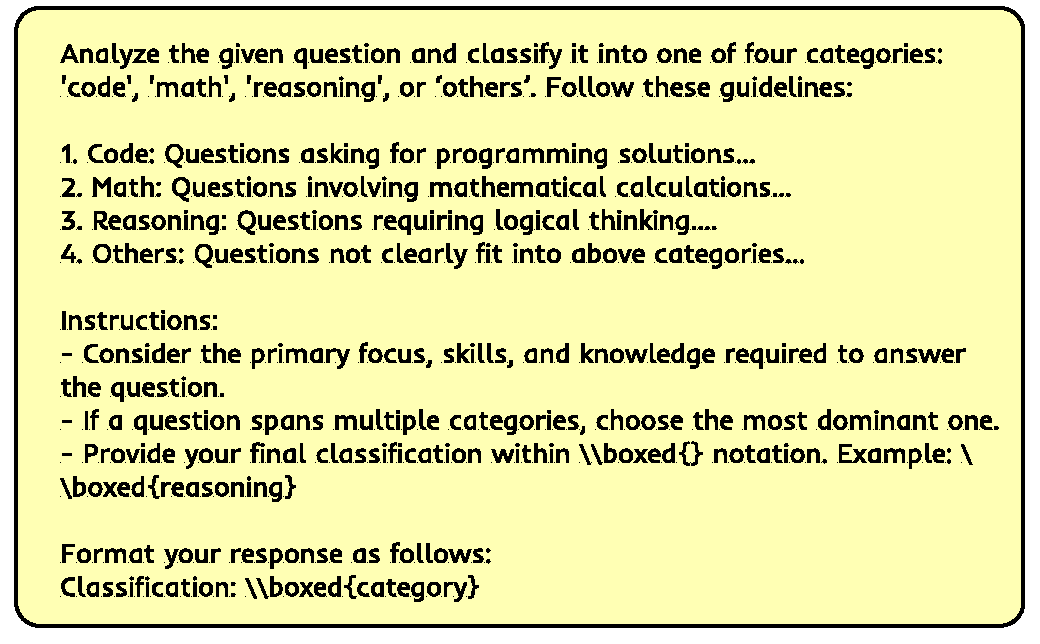
\includegraphics[width=0.45\textwidth]{images/visualization/system_prompt.pdf}
  \end{center}
  \vspace{-5.5mm} 
  \caption{\textbf{Prompt based adaptation.} Self-adaptation prompt used by \implname to classify the task prompt into pre-defined categories.}
  \label{fig:sys_prompt}
  \vspace{-4mm}
\end{wrapfigure}

\textit{B) Classification expert:} 
A direct extension of the prompt engineering approach comes from using a specialized system to handle task identification.
Following the principles of self-adaptation, we apply \svdacro to fine-tune the base LLM itself to handle this task.
In particular, we collect a dataset $D = \{(x_{1,1}, 1), \cdots, (x_{i,k}, k), \cdots \}$ from the $K$ \svdacro training tasks, where $x_{i,k}$ is the $i$-th example from the $k$-th expert task.
Each tuple $(x_{i,k}, k)$ then forms an example to pre-train an additional job classification expert $z^c$ learned in the same fashion as the others.
During the first inference pass, we simply load $z^c$, intending to improve the inherent task classification capabilities of the base model to select a more appropriate $z'$ to handle the input prompt. 

\textit{C) Few-shot adaptation:} Our third approach leverages additional task information by assuming extended access to its test-time conditions beyond individual prompts. 
Our approach is inspired by popular few-shot prompting techniques, which have been shown to provide consistent performance improvements and even allow LLMs to ``in-context'' learn tasks that were entirely unseen prior to inference~\citep{brown2020language}.
For each optimized $W$, our approach entails producing an entirely new $z^\prime=\sum^{K}_{k=1} \alpha_k z_k$ by linearly interpolating between the $K$ learned \svdacro vectors, each weighted by the coefficients $\alpha_k$.
We employ CEM to search over the possible values of each $\alpha_k$ based on the performance on a set of ``few-shot prompts'', which are specifically held out from the rest of the test prompts and used to evaluate CEM's population samples. 
In the case of multiple population samples obtaining the same score on these held-out prompts, we break ties by favoring the one with the highest average log-likelihood across its own generated correct answers.
Crucially, we only need to perform this process once for each target task, avoiding the need to increase the length of each question prompt, a relevant downside of traditional few-shot prompting. We refer to Section~\ref{app:sec:fewshot}, for additional details and an extended discussion of this final approach. 

\vspace{-2mm}
\section{Experiments}
\label{sec:experiments}

\vspace{-2mm}

We extensively evaluate \implname on multiple tasks and models with the purpose of:
(1) assessing the efficiency and effectiveness of \svdacro;
(2) demonstrating self-adaptiveness through the three proposed adaptation strategies;
(3) conducting in-depth analysis and ablation studies aimed at understanding and interpreting the properties of our new framework.

\vspace{-2mm}
\subsection{Experimental setups}
\vspace{-1mm}

To validate the generality of \implname we consider three pre-trained LLMs ranging across different model families and architecture sizes: \llama, \mistral, and \llamaXL.
For each model, we obtain three sets of \svdacro-trained $z$ vectors to maximize performance for GSM8K~\citep{cobbe2021training},  MBPP-pro~\citep{austin2021program}, and ARC-Easy~\citep{clark2018think}, respectively.
Additionally, we also train a set of $z$ vectors for \llama, when applied as the language backbone for TextVQA~\citep{singh2019towards}, in order to assess \svdacro's applicability to the vision-language modeling (VLM) domain.
We provide \svdacro's main learning curves on each of these tasks in Figure~\ref{fig:learning_curves}. 
Finally, we evaluate the full \implname adaptation framework on four unseen tasks: MATH~\citep{hendrycks2021measuring}, Humaneval~\citep{chen2021evaluating}, ARC-Challenge~\citep{clark2018think}, and OKVQA~\citep{marino2019ok}. In all our adaptation experiments, we only consider experts obtained in the pure-language settings, assessing its test-time applicability even for the distinctive vision domain. 
Please refer to the Appendix~\ref{app:sec:implementation} for additional details and a summary of the hyper-parameters used in the experiments.

\begin{figure}[!t]
    \centering
    % \vspace{-4mm}
    \includegraphics[width=0.95\textwidth]{images/learning_curves_new.pdf}
    \vspace{-4mm}
    \caption{\textbf{\svdacro learning curves.} The dashed lines indicate the performance of \llama on the test split of each task. SVF effectively fine-tunes to surpass the base performance. While we use the best validation score to select our checkpoint for evaluation (marked by red dots), we present the entire training curve without early stopping to demonstrate \svdacro's learning capabilities. Tasks with only hundreds of training samples like Coding and Reasoning were stopped early. In our experiments, we update the parameters at the end of each epoch.}
    \vspace{-6mm}
    \label{fig:learning_curves}
\end{figure}


\subsection{Experimental results}

% \begin{table}[!t]
% \centering

% \caption{\textbf{LLM Fine-tuning Results.} LLM performance on the test splits.}

% \small
% \begin{tabular}{llll}
% \toprule

% \textbf{Method} & \textbf{GSM8K} & \textbf{MBPP-Pro} & \textbf{ARC-Easy} \\

% \midrule
% \llama & {\normalsize 75.89 {\footnotesize (\grey{1.00})}} & {\normalsize 64.65 {\footnotesize (\grey{1.00})}} & {\normalsize 88.59 {\footnotesize (\grey{1.00})}} \\
% \quad + LoRA & {\normalsize 70.58 {\footnotesize (\red{0.93})}} & \textbf{{\normalsize 67.68 {\footnotesize (\green{1.05})}}} & {\normalsize 88.97 {\footnotesize (\grey{1.00})}} \\
% \quad + SVF (Ours) & \textbf{{\normalsize 79.15 {\footnotesize (\green{1.04})}}} & {\normalsize 66.67 {\footnotesize (\green{1.03})}} & \textbf{{\normalsize 89.56 {\footnotesize (\green{1.01})}}} \\

% \midrule
% \mistral & {\normalsize 42.83 {\footnotesize (\grey{1.00})}} & {\normalsize 49.50 {\footnotesize (\grey{1.00})}} & {\normalsize 49.50 {\footnotesize (\grey{1.00})}} \\
% \quad + LoRA & {\normalsize 36.09 {\footnotesize (\red{0.84})}} & {\normalsize 47.47 {\footnotesize (\red{0.96})}} & {\normalsize 47.47 {\footnotesize (\red{0.96})}} \\
% \quad + SVF (Ours) & \textbf{{\normalsize 49.74 {\footnotesize (\green{1.16})}}} & \textbf{{\normalsize 51.52 {\footnotesize (\green{1.04})}}} & \textbf{{\normalsize 85.14 {\footnotesize (\green{1.72})}}} \\

% \midrule
% \llamaXL & {\normalsize 85.29 {\footnotesize (\grey{1.00})}} & \textbf{{\normalsize 80.81 {\footnotesize (\grey{1.00})}}} & \textbf{{\normalsize 89.10 {\footnotesize (\grey{1.00})}}} \\
% \quad + SVF (Ours) & \textbf{{\normalsize 88.32 {\footnotesize (\green{1.04})}}} & \textbf{{\normalsize 80.81 {\footnotesize (\grey{1.00})}}} & {\normalsize 88.47 {\footnotesize (\red{0.99})}} \\

% \bottomrule
% \end{tabular}

% \label{tab:res:svf_train_tasks}
% \end{table}

% \begin{figure}[!t]
%     \centering
%     \includegraphics[width=\textwidth]{images/vlm_barplot.pdf}
%     % \vspace{-8mm}
%     \caption{\textbf{VLM Results.}
%     }
%     % \vspace{-4mm}
%     \label{fig:vlm_results}
% \end{figure}



\begin{figure}[!b]
    \vspace{-4mm}
    \centering

    % Left side: Table
    \begin{minipage}{0.75\linewidth}
        \centering
        \captionof{table}{\textbf{Fine-tuning results.} LLM performance on the test splits of math, coding and reasoning. Normalized scores are in the parentheses.}
        \vspace{-2mm}
        \small
        \begin{tabular}{llll}
            \toprule
            \textbf{Method} & \textbf{GSM8K} & \textbf{MBPP-Pro} & \textbf{ARC-Easy} \\
            \midrule
            \llama & {\normalsize 75.89 {\scriptsize (\grey{1.00})}} & {\normalsize 64.65 {\scriptsize (\grey{1.00})}} & {\normalsize 88.59 {\scriptsize (\grey{1.00})}} \\
            \quad + LoRA & {\normalsize 70.58 {\scriptsize (\red{0.93})}} & \textbf{{\normalsize 67.68 {\scriptsize (\green{1.05})}}} & {\normalsize 88.97 {\scriptsize (\grey{1.00})}} \\
            \quad + SVF (Ours) & \textbf{{\normalsize 79.15 {\scriptsize (\green{1.04})}}} & {\normalsize 66.67 {\scriptsize (\green{1.03})}} & \textbf{{\normalsize 89.56 {\scriptsize (\green{1.01})}}} \\
            \midrule
            \mistral & {\normalsize 42.83 {\scriptsize (\grey{1.00})}} & {\normalsize 49.50 {\scriptsize (\grey{1.00})}} & {\normalsize 49.50 {\scriptsize (\grey{1.00})}} \\
            \quad + LoRA & {\normalsize 36.09 {\scriptsize (\red{0.84})}} & {\normalsize 47.47 {\scriptsize (\red{0.96})}} & {\normalsize 47.47 {\scriptsize (\red{0.96})}} \\
            \quad + SVF (Ours) & \textbf{{\normalsize 49.74 {\scriptsize (\green{1.16})}}} & \textbf{{\normalsize 51.52 {\scriptsize (\green{1.04})}}} & \textbf{{\normalsize 85.14 {\scriptsize (\green{1.72})}}} \\
            \midrule            
            \llamaXL & {\normalsize 85.29 {\footnotesize (\grey{1.00})}} & \textbf{{\normalsize 80.81 {\footnotesize (\grey{1.00})}}} & \textbf{{\normalsize 89.10 {\footnotesize (\grey{1.00})}}} \\
            \quad + LoRA & {\normalsize 77.26 {\footnotesize (\red{0.91})}} & {\normalsize 68.69 {\footnotesize (\red{0.85})}} & {\normalsize 88.55 {\footnotesize (\red{0.99})}} \\
            \quad + SVF (Ours) & \textbf{{\normalsize 88.32 {\footnotesize (\green{1.04})}}} & \textbf{{\normalsize 80.81 {\footnotesize (\grey{1.00})}}} & {\normalsize 88.47 {\footnotesize (\red{0.99})}} \\
            \bottomrule                
        \end{tabular}
        \label{tab:res:svf_train_tasks}
    \end{minipage}
    \hfill
    % Right side: Figure
    \begin{minipage}{0.23\linewidth}
        \centering
        % \vspace{2mm}
        \includegraphics[width=\linewidth]{images/vlm_barplot.pdf}
        \vspace{-8mm}
        \captionof{figure}{\textbf{Results for the VLM domain.}}
        \label{fig:vlm_results}
    \end{minipage}

\end{figure}


\textbf{\svdacro performance}
We provide results after training on each considered task with the \llama, \mistral, and \llamaXL base models in Table~\ref{tab:res:svf_train_tasks}.
Remarkably, we find that \svdacro provides considerable and consistent performance gains across nearly all tasks and base models. Instead, LoRA experts yield smaller gains and even sporadic performance degradation.
(These LoRA experts are trained with next token prediction. While we also have LoRA experts trained with RL in Table~\ref{tab:res:ablation}, RL seems work less well with LoRA than with \svdacro.)
This observed trend extends also to the vision-language domain, as fine-tuning \textsc{Llama3-Llava-Next-8B} with \svdacro bolsters the base model's performance by over 39\% (see Figure~\ref{fig:vlm_results}).
To ensure a fair comparison, we provide extensive ablations to both our model and the LoRA baseline considering different architecture and optimization objectives in Appendix~ \ref{app:sec:ablation_studies}).
Due to its essential parameterization, we would like to note that training \svdacro requires considerably fewer resources, with less than 10\% of the training parameters of our LoRA implementation.

\textbf{Adaptation performance}
With the \svdacro trained $z$ vectors, we assess the self-adaptation capability of \implname on unseen tasks.
For a fair comparison with LoRA, we record the performance of this baseline using all checkpoints from the considered training tasks and report only its highest performance for each of the test tasks. 
As shown in Table~\ref{tab:res:svf_ada_tasks}, all of our \implname adaptation strategies demonstrate improvements across all tasks for \llama base models, and in at least two out of three tasks for both \mistral and \llamaXL.
In contrast, even the best training LoRAs only provide marginal improvements on the ARC-Challenge task and still significantly deteriorate performance on both MATH and Humaneval. 
This discrepancy suggests that LoRA's parameterization and optimization might be particularly sensitive to overfitting, especially when trained with the smaller GSM8K and MBPP-Pro datasets, the tasks that provide information most related to MATH and Humaneval.
In Figure~\ref{fig:vlm_results}, we find a similar dichotomy in the OKVQA task, with the performance of the base \textsc{Llama3-Llava-Next-8B} VLM only improving after applying \implname.
We note that also in this setting, \implname performs self-adaptation only from the expert vectors from GSM8K, MBPP-Pro, and ARC-Easy.
Thus, this result further underscores the high flexibility of self-adaptation, transferring knowledge compressed for tasks entirely based on language even for unrelated vision-based problems.

\begin{table}[!t]
\centering
\vspace{-2mm}
\caption{\textbf{Self-adaptation on unseen tasks.} Normalized scores are in the parentheses.}
% \vspace{-2mm}
\small
\begin{tabular}{llll}
\toprule
Method & MATH & Humaneval & ARC-Challenge \\

\midrule
\llama3 & {\normalsize 24.54 {\footnotesize (\grey{1.00})}} & {\normalsize 60.98 {\footnotesize (\grey{1.00})}} & {\normalsize 80.63 {\footnotesize (\grey{1.00})}} \\
\quad + LoRA & {\normalsize 21.68 {\footnotesize (\red{0.88})}} & {\normalsize 52.44 {\footnotesize (\red{0.86})}} & {\normalsize 81.06 {\footnotesize (\green{1.01})}} \\
\quad + \implname (Prompt) & {\normalsize 25.22 {\footnotesize (\green{1.03})}} & {\normalsize 61.59 {\footnotesize (\green{1.01})}} & {\normalsize 81.74 {\footnotesize (\green{1.01})}} \\
\quad + \implname (Cls-expert) & {\normalsize 25.18 {\footnotesize (\green{1.03})}} & {\normalsize 62.80 {\footnotesize (\green{1.03})}} & {\normalsize 81.37 {\footnotesize (\green{1.01})}} \\
\quad + \implname (Few-shot) & \textbf{{\normalsize 25.47 {\footnotesize (\green{1.04})}}} & \textbf{{\normalsize 62.99 {\footnotesize (\green{1.03})}}} & \textbf{{\normalsize 82.61 {\footnotesize (\green{1.02})}}} \\

\midrule
\mistral & {\normalsize 13.02 {\footnotesize (\grey{1.00})}} & {\normalsize 43.29 {\footnotesize (\grey{1.00})}} & {\normalsize 71.76 {\footnotesize (\grey{1.00})}} \\
\quad + LoRA & {\normalsize 11.18 {\footnotesize (\red{0.86})}} & {\normalsize 31.71 {\footnotesize (\red{0.73})}} & \textbf{{\normalsize 75.77 {\footnotesize (\green{1.06})}}} \\
\quad + \implname (Prompt) & {\normalsize 11.86 {\footnotesize (\red{0.91})}} & {\normalsize 43.90 {\footnotesize (\green{1.01})}} & {\normalsize 72.35 {\footnotesize (\green{1.01})}} \\
\quad + \implname (Cls-expert) & {\normalsize 11.60 {\footnotesize (\red{0.89})}} & {\normalsize 43.90 {\footnotesize (\green{1.01})}} & {\normalsize 74.83 {\footnotesize (\green{1.04})}} \\
\quad + \implname (Few-shot) & \textbf{{\normalsize 13.39 {\footnotesize (\green{1.03})}}} & \textbf{{\normalsize 47.40 {\footnotesize (\green{1.09})}}} & {\normalsize 75.47 {\footnotesize (\green{1.05})}} \\

\midrule
\llamaXL & \textbf{{\normalsize 40.64 {\footnotesize (\grey{1.00})}}} & {\normalsize 78.66 {\footnotesize (\grey{1.00})}} & {\normalsize 87.63 {\footnotesize (\grey{1.00})}} \\
\quad + LoRA & {\normalsize 25.40 {\footnotesize (\red{0.62})}} & {\normalsize 73.78 {\footnotesize (\red{0.94})}} & {\normalsize 83.70 {\footnotesize (\red{0.96})}} \\
\quad + \implname (Prompt) & {\normalsize 40.44 {\footnotesize (\grey{1.00})}} & \textbf{{\normalsize 79.88 {\footnotesize (\green{1.02})}}} & \textbf{{\normalsize 88.48 {\footnotesize (\green{1.01})}}} \\
\bottomrule

\end{tabular}

\label{tab:res:svf_ada_tasks}
\vspace{-6mm}
\end{table}



Comparing the three proposed adaptation strategies, we highlight a clear monotonic trend -- with more involved strategies and additional information about the test-time condition, self-adaptation appears to be increasingly effective.
In particular, \implname with few-shot self-adaptation is almost always the highest-scoring method, providing notable improvements across all tested settings except for \llamaXL@MATH, where we have only SVF-tuned half of the layers due to our limited GPU resources.
This trend shows that providing additional or different kinds of information seems to be highly beneficial to our framework, suggesting that \implname could provide foundation models with new means to continually improve performance when deployed in lifelong settings.

\begin{wraptable}{r}{0.35\textwidth}
\vspace{-6mm}
\centering
\caption{\textbf{Time cost of 2-pass inference in prompt adaptation strategy of \implname for the entire problem set.} 1st to 2nd pass inference time ratios are shown in parentheses.}
\label{tab:res:inference_time}
\vspace{-3.5mm}
\small
\resizebox{0.35\textwidth}{!}{
\begin{tabular}{lrr}
\toprule
\textbf{Task} & \textbf{1st (s)} & \textbf{2nd (s)} \\
\midrule
MATH         & 42.64    {\footnotesize (13\%)}             & 321.19                  \\
Humaneval    & 2.76   {\footnotesize (19\%)}                 & 14.28                   \\
ARC-Challenge & 13.40      {\footnotesize (47\%)}             & 28.51                   \\
\bottomrule
\end{tabular}
}
\vspace{-4mm}
\end{wraptable}

Table~\ref{tab:res:inference_time} reports the inference time required by the prompt adaptation strategy of \implname, with the time spent on solving the entire problem set presented separately for the 1st and 2nd passes.
Notice that the 2nd pass inference time is the time spent on solving the problems, and the 1st pass inference time is the time for self-adaptation, 1st to 2nd pass inference time ratios are in the parentheses.
While the additional inference pass might appear to double the overall runtime, it is important to note that inference time primarily depends on the number of tokens generated.
In our settings, it is $\mathcal{O}(n)$ where $n$ is the length of the input.
ARC-challenge's cost ratio is large because they are single choice problems and therefore the cost of the 2nd pass is also $\mathcal{O}(n)$.
In general settings, we think it is reasonable to assume this ratio to be closer to those of MATH and Humaneval.
For a detailed discussion on improving the efficiency of CEM few-shot adaptation methods, please see Appendix~\ref{app:sec:efficiency_improvements}

\subsection{Analysis}
\label{sec:analysis}

Lastly, we analyze and discuss the properties of our adaptation strategies for which we provide extensions and further discussion Appendix~\ref{app:sec:additional_exp}.

\textbf{Analysis 1: Job dispatching accuracy}
In Figure~\ref{fig:confusion_matrices} we provide the confusion matrices of our classification-based adaptation strategies. These results validate the effectiveness of both our classification-based adaptation strategies to match each prompt with experts trained in similar domains, as evidenced by the high values along the diagonals. 
Furthermore, the results from \llama and \mistral also show that using the classification expert consistently provides higher classification accuracy than vanilla prompt engineering.
While this difference could explain the higher performance of the relative self-adaptation strategy, we also note that domain similarity might not be the only metric relevant to identifying the best expert for each prompt or task.
To this end, we believe many further unexplored extensions could be explored in future work, using heuristics such as past expert performance or token-level analysis to further push our framework's scalability.

\begin{figure}[t]%[!b]
    \centering
    \vspace{-0.5mm}
    \includegraphics[width=0.9\textwidth]{images/confusion_matrices.pdf}
    \vspace{-4mm}
    \caption{\textbf{Confusion matrices.} These matrices display the classification percentages, where rows represent the task classes (ground truth) and columns indicate the predicted categories. Some samples are misclassified as ``Others,'' which is reflected in rows where the totals do not sum to one.
    }
    \vspace{-10mm}
    \label{fig:confusion_matrices}
\end{figure}

\textbf{Analysis 2: Training tasks adaptation contribution}
In Figure~\ref{fig:cem}, we show the normalized adaptive coefficients $a_k$ interpolating between our \svdacro vectors learned via CEM for \llama and \mistral across all the unseen downstream tasks. 
Intuitively, we find that the expert vectors from the training tasks sharing similar topics to the unseen ones are often the highest contributors to the produced adaptive weights. 
However, we observe that the MATH task appears as an interesting exception, as the $a_k$ for the expert obtained from GSM8K training is actually the lowest out of the three in both models.
We hypothesize this reflects the different nature of the mathematics competition problems from MATH as compared to the grade-school problems in GSM8K.
In fact, not only is the difficulty of the MATH questions far beyond GSM8K, but a large portion of its problems also hinges mainly on logical reasoning, for which a task like ARC might actually be more aligned.
Furthermore, we also note that the different $z$ vectors appear to contribute more uniformly to adaptation in the Llama model.
This difference might indicate that, due to its higher base performance, the Llama model does not need to rely on any particular set of skills as much as Mistral, and can harness more holistic benefits from self-adaptation.
Note that applying $a_k$ uniformly is not a universal solution for leveraging expert vectors. This becomes evident when we look at different model and task combinations (e.g. applying $a_k$ uniformly on \llama for MATH tasks only achieves 24.47, while \implname(Few-shot) achieves 25.47).

\textbf{Analysis 3: Ablation studies}

\label{app:sec:ablation_studies}

\textit{Module sensitivity:} We first compare the performance of \svdacro when it is applied to different modules (see trials 1-3).
Under consistent conditions, both individual MLP and attention updates improve performance, with MLP updates resulting in more pronounced gains.
Simultaneous updates to both module types yield even more significant enhancements.

\textit{Objective function:} We are interested in the performance impact from different objective functions, and we compare the RL objective with next-token prediction loss (see trials 2 and 4).
For the latter, we use instruction fine-tuning with official GSM8K solutions as target tokens.
Results show clear performance gains with RL, demonstrating its effectiveness in task-specific fine-tuning.
Conversely, next-token prediction even hinders performance.
This highlights RL's ability to handle cases lacking detailed solutions, suggesting its superiority in this context.

\textit{\svdacro vs LoRA:} Finally, we also evaluate LoRA using the RL objective (see trials 2 and 5).
A significant performance disparity is observed, primarily attributed to the severe instability of the LoRA training process.
Despite exploring a wide range of learning rates, LoRA's performance consistently lagged behind.
For further illustrations, see Figure~\ref{app:fig:lora_learning_curves} in the appendix.
\begin{table}[h]
% \begin{table}[!b]

% \vspace{-2mm}
\centering
\caption{\textbf{Ablation studies.} We fine-tune \llama on the GSM8K training split with different settings and the results on the test split along with zero-shot transfer results on MATH.
% We highlight the change in learning configurations for better visualization.
%Notably, we set the KL coefficient to 0.1 across all runs utilizing policy gradient for fair comparison.
}
% \vspace{-3.5mm}
% \small
% \begin{tabular}{llllccc}
% \toprule

% \textbf{\#} & \textbf{Method} & \textbf{Objective Function} & \textbf{Module} & \textbf{\#Params ($\downarrow$)} & \textbf{GSM8K ($\uparrow$)} & \textbf{MATH ($\uparrow$)} \\

% \midrule
% 0 & \multicolumn{4}{c}{\textsc{LLAMA-3-8B-Instruct}} & {75.89 {\scriptsize (\grey{1.00})}} & {24.54 {\scriptsize (\grey{1.00})}} \\ 
% \midrule

% 1 & \svdacro & Policy gradient & MLP & 0.39M & { 78.62 {\scriptsize (\green{1.04})}} & {24.20 {\scriptsize (\green{0.99})}} \\

% 2 & \svdacro & Policy gradient & \cellcolor{gray!20}{attention} & \textbf{0.16M} & {76.19 {\scriptsize (\green{1.00})}} & {24.20 {\scriptsize (\green{0.99})}} \\

% 3 & \svdacro & Policy gradient & \cellcolor{gray!20}{MLP + attention} & 0.58M & \textbf{{ 79.23 {\scriptsize (\green{1.04})}}} & \textbf{{25.04 {\scriptsize (\green{1.04)}}}} \\

% 4 & \svdacro & \cellcolor{gray!20}{Next token pred} & attention & \textbf{0.16M} & { 60.50 {\scriptsize (\green{0.80})}} & {18.52 {\scriptsize (\green{0.75})}} \\

% 5 & \cellcolor{gray!20}{LoRA} & Policy gradient & attention & 6.82M & { 57.92 {\scriptsize (\green{0.76})}} & {15.72 {\scriptsize (\green{0.64})}} \\

% \bottomrule
% \label{tab:res:ablation}
% \end{tabular}

% \vspace{-8mm}
% \end{table}

% \vspace{-3.5mm}
\small
\begin{tabular}{llllccc}
\toprule

\textbf{\#} & \textbf{Method} & \textbf{Objective Function} & \textbf{Module} & \textbf{\#Params ($\downarrow$)} & \textbf{GSM8K ($\uparrow$)} & \textbf{MATH ($\uparrow$)} \\

\midrule
0 & \multicolumn{4}{c}{\textsc{LLAMA-3-8B-Instruct}} & {75.89 {\scriptsize (\grey{1.00})}} & {24.54 {\scriptsize (\grey{1.00})}} \\ 
\midrule

1 & \svdacro & Policy gradient & MLP & 0.39M & { 78.62 {\scriptsize (\green{1.04})}} & {24.20 {\scriptsize (\green{0.99})}} \\

2 & \svdacro & Policy gradient & attention & \textbf{0.16M} & {76.19 {\scriptsize (\green{1.00})}} & {24.20 {\scriptsize (\green{0.99})}} \\

3 & \svdacro & Policy gradient & MLP + attention & 0.58M & \textbf{{ 79.23 {\scriptsize (\green{1.04})}}} & \textbf{{25.04 {\scriptsize (\green{1.04)}}}} \\

4 & \svdacro & Next token pred & attention & \textbf{0.16M} & { 60.50 {\scriptsize (\green{0.80})}} & {18.52 {\scriptsize (\green{0.75})}} \\

5 & LoRA & Policy gradient & attention & 6.82M & { 57.92 {\scriptsize (\green{0.76})}} & {15.72 {\scriptsize (\green{0.64})}} \\

\bottomrule
\label{tab:res:ablation}
\end{tabular}

\vspace{-5mm}
\end{table}



\textbf{Analysis 4: Cross-model compatibility}
Finally, we explore the potential for our self-adaptation framework to be applied \textit{across different LLMs}.  In particular, we evaluate whether the \svdacro expert vectors trained on \llama can benefit \mistral, and whether we can perform adaptation across the expert vectors of these two models. We present our main findings in Table~\ref{tab:analysis:cross_model_main} and refer to Appendix~\ref{app:sec:additional_exp} for additional detailed results. 
Surprisingly, we find that positive transfer occurs across the two models, with visible benefits in 2 out of 3 tasks.
We note these improvements are due to the inherent ordering of the \svdacro parameterization, as \textit{randomly shuffling} each \svdacro vector before applying it to the Mistral model consistently degrades performance.

\begin{wrapfigure}{r}{0.32\textwidth}
\vspace{-12mm}
\begin{center}
    \includegraphics[width=0.32\textwidth]{images/cem_plot_vertical_tb.pdf}
  \end{center}
  \vspace{-10mm}
  \caption{\textbf{$\boldsymbol{\alpha_k}$ learned weights.}}
  \label{fig:cem}
  \vspace{-4mm}
\end{wrapfigure}

This operation leads to notable performance degradation across each task. 
Finally, by performing few-shot adaptation using the \svdacro vectors collected from both models, the performance of \mistral further improves across the board.
We observe that these gains even surpass the best score from adapting \mistral with \textit{all} the \svdacro vectors in the ARC-Challenge task reported in Table~\ref{tab:res:svf_ada_tasks}.  
While these results appear promising, we note that the surprising compatibility discovered through our naive transfer approach is potentially tied to the similarity between the architectures of the two considered LLMs.
To this end, whether similar transfer can be replicated with models of different scales remains an open research question that could open the doors to disentangling and recycling task-specific skills for newer/larger models, with important implications for democratization and sustainability.

\begin{table}[!h]
% \vspace{-4mm}
% \caption{\textbf{Cross-model $z$ vector transfer.}
\caption{\textbf{Cross-model $\boldsymbol{z}$ vector transfer.}
Results from transferring the expert vectors trained on \llama to \mistral with cross model few-shot adaptation.
}
% \vspace{-3.5mm}
\centering
\begin{tabular}{lccc}
\toprule
\textbf{Method} & \textbf{MATH} & \textbf{Humaneval} & \textbf{ARC-Challenge} \\
\textit{SVF training task} & \small{\textit{GSM8K}} & \small{\textit{MBPP-pro}} & \small{\textit{ARC-Easy}} \\
\midrule


\textsc{Mistral-7B-Instruct-v0.3} & \textbf{{\normalsize 13.02 {\footnotesize (\grey{1.00})}}} & {\normalsize 43.29 {\footnotesize (\grey{1.00})}} & {\normalsize 71.76 {\footnotesize (\grey{1.00})}} \\

\midrule

\quad + Llama SVF (ordered $\sigma_i$) & {\normalsize 11.96 {\footnotesize (\red{0.92})}} & {\normalsize 45.12 {\footnotesize (\green{1.04})}} & {\normalsize 72.01 {\footnotesize (\grey{1.00})}} \\
\quad + Llama SVF (shuffled $\sigma_i$) & {\normalsize 10.52 {\footnotesize (\red{0.81})}} & {\normalsize 40.24 {\footnotesize (\red{0.93})}} & {\normalsize 70.82 {\footnotesize (\red{0.99})}} \\
\quad + Few-shot adaptation (cross-model) & {\normalsize 12.65 {\footnotesize (\red{0.97})}} & \textbf{{\normalsize 46.75 {\footnotesize (\green{1.08})}}} & \textbf{{\normalsize 75.64 {\footnotesize (\green{1.05})}}} \\

\bottomrule
\end{tabular}
\label{tab:analysis:cross_model_main}
\vspace{-2mm}
\end{table}

\vspace{-1mm}
\section{Conclusion}
\label{sec:conclusion}
\vspace{-3mm}

In this paper, we introduced \implname, providing a novel blueprint toward realizing self-adaptive LLMs.
Within this framework, we first proposed \svdacro, offering superior performance than prior fine-tuning recipes, together with reduced costs, high compositionality, and overfitting regularization -- all crucial properties to achieve scalable self-adaptation.
Leveraging a set of \svdacro experts as building blocks, we developed three effective strategies for self-adaptation, each offering unique benefits and monotonic performance benefits with increasing access to the test-time conditions.

While \implname demonstrates promising results, there remain exciting opportunities for future work.
One limitation is that the capabilities of \svdacro experts are tied to the latent components of the base model.
To address this, model merging offers a promising direction~\citep{yu2024language,goddard2024arcee,akiba2024evolutionary}, enabling specialized models to be combined into a single, more capable model.
Additionally, while our CEM-based adaptation effectively balances performance and efficiency, scaling to a large number of specialized domains may introduce increased one-time computational costs.
However, this trade-off is offset by the benefits of improved performance and enhanced self-adaptation capabilities.
Advances in model merging and efficient adaptation techniques have produced models dominating open leaderboards, making them strong candidates as base models for \implname and opening new possibilities for adaptive LLMs.

\ificlrfinal

\section{Author contributions}

Yujin Tang initiated the project.
Qi Sun proposed the prompted-based method, developed the evaluation framework, conducted the experiments, and provided contributions to writing.
Edoardo Cetin designed the few-shot CEM adaptation strategy, performed the experiment, and made major contributions to manuscript writing.
Yujin Tang proposed the core algorithm, conducted initial experiments, made major contributions to the manuscript, and managed the project.

\fi

\bibliography{ref}
\bibliographystyle{iclr2025_conference}

\newpage
\section{Appendix} \label{appendix}


\subsection{NewYorker Data for evaluation}

\begin{figure}[!ht]
\small
\centering
\includegraphics[width=0.4\textwidth]{figures/length.png}
\caption{\label{lengthdist} Distribution of word count of stories in our test set}
\end{figure}

Table \ref{teststories} shows the data used for conducting our evaluation. The 12 stories shown are taken from The New Yorker and summarized into single-sentence plots. These stories come from highly established literary experts acting as an upper bound for what it means to be creative. These stories span complex themes.

\begin{table*}[!ht]
\centering
\small
\def\arraystretch{1.35}
\begin{tabular}{|l|}
\hline
\begin{tabular}[c]{@{}l@{}}Write a New Yorker-style story given the plot below. Make sure it is atleast \textbf{\color{blue}\{\{word\_count\}\}} words. Directly start with the\\ story, do not say things like `Here's the story {[}...{]}:\end{tabular}                                                                                                                                                                                            \\ \hline\hline
\begin{tabular}[c]{@{}l@{}}You wrote the story I gave you below. I requested a story with \textbf{\color{blue}\{\{word\_count\}\}} words, but the story only has\\ \textbf{\color{blue}\{\{current\_word\_count\}\}} words. Can you rewrite the story to make it longer, and closer to the \textbf{\color{blue}\{\{word\_count\}\}} word target\\ I gave you. Directly start with the story, do not say things like `Here's the story {[}...{]}:`\\ \\ Current story: \{\{story\}\}\end{tabular} \\ \hline
\end{tabular}
\vspace{2ex}
\caption{\label{promptstory}Prompt to write the initial story (Row1) vs Prompt to rewrite the initial story to be longer. word\_count represents the number of words in the human written story on a given plot (P) while current\_word\_count represents the number of words in the LLM generated story on the same plot (P)}
\end{table*}

\begin{table*}[!ht]
\def\arraystretch{1.15}
\small
\begin{tabular}{|l|l|}
\hline
Story                                    & Plot                                                                                                                                                                                                                                                                                                                                                                                                                                                                                                                                   \\ \hline
\href{https://www.newyorker.com/books/flash-fiction/a-triangle}{A Triangle}                               & \begin{tabular}[c]{@{}l@{}}An observer becomes entranced by a seemingly ordinary couple on the street, follows them home, and then \\watches them from outside in the rising floodwaters, drawing an eerie connection between the woman and\\ a discarded, burned chair they'd noticed earlier.\end{tabular}                                                                                                                                                                    \\ \hline\hline
\href{https://www.newyorker.com/books/flash-fiction/barbara-detroit-1966}{\begin{tabular}[c]{@{}l@{}}Barbara\\ Detroit,1966\end{tabular}}                    & \begin{tabular}[c]{@{}l@{}}On Feb 12, 1966, a heavily pregnant woman named Barbara experienced a shocking incident in her synagogue\\in Southfield, Detroit, where a young man shot and killed the renowned Rabbi Adler before turning the gun\\ on himself, and though Barbara tried to reach the shooter, she was swept away by the fleeing crowd.\end{tabular}                                                                              \\ \hline\hline
\href{https://www.newyorker.com/books/flash-fiction/beyond-nature}{Beyond Nature}                           & \begin{tabular}[c]{@{}l@{}}A solitary man walking in a remote mountainous region comes across a car crash, and stays by the side\\ of the lifeless female victim, narrating stories of his past and reflecting on the impermanence of \\events and life itself, while awaiting emergency services amidst the looming presence of wilderness.\end{tabular}                                                                                                                \\ \hline\hline
\href{https://www.newyorker.com/books/flash-fiction/certain-european-movies}{\begin{tabular}[c]{@{}l@{}}Certain European\\ Movies\end{tabular}}                  & \begin{tabular}[c]{@{}l@{}}Two individuals, at a residency together, navigate the complexity of their ephemeral relationship during\\ their final beach trip, framed by misadventures, subtle tensions, unspoken desires, and looming departures.\end{tabular}                                                                                                                                                                                   \\ \hline\hline
\href{https://www.newyorker.com/books/flash-fiction/keys}{Keys}                                     & \begin{tabular}[c]{@{}l@{}}Daniel, struggling with recurring dreams of his ex-wife Rachel and a mysterious unused flat, eventually \\discusses them with his current partner Isabel, sparking various reflections and conversations about their\\ past relationships, until a real-life discovery of old keys triggers a nostalgic memory and helps him find a\\ way to reconnect with his present relationship through canoeing.\end{tabular}                                     \\ \hline\hline
\href{https://www.newyorker.com/books/flash-fiction/listening-for-the-click}{\begin{tabular}[c]{@{}l@{}}Listening For\\ the Click\end{tabular}}                  & \begin{tabular}[c]{@{}l@{}}Navigating a complex social landscape, the protagonist experiences a series of complex relationships \\and emotional turmoil in a student environment, and engages in self-discovery and self-reflection as she\\ interacts with the characters Carl, Martin, Lizzy, and Johan, resulting in a journey of introspection,\\ betrayal, love, and personal growth.\end{tabular}                                                          \\ \hline\hline
\href{https://www.newyorker.com/magazine/2023/05/15/maintenance-hvidovre-fiction-olga-ravn}{\begin{tabular}[c]{@{}l@{}}Maintenance,\\ Hvidovre\end{tabular}}                   & \begin{tabular}[c]{@{}l@{}}A woman experiences a disorienting night in a maternity ward where she encounters other similarly \\disoriented new mothers, leading to an uncanny mix-up where she leaves the hospital with a baby \\that she realizes is not her own, yet accepts the situation with an inexplicable sense of happiness.\end{tabular}                                                                                                  \\ \hline\hline
\href{https://www.newyorker.com/magazine/2022/11/14/returns}{Returns}                                  & \begin{tabular}[c]{@{}l@{}}The narrator visits their elderly mother in her small town, spending a day with her that is filled with \\nostalgia, conversation, and old habits, only to return a month later after her hospitalization due to\\ a sunstroke, finding remnants of their last visit.\end{tabular}                                                                                                                                                                      \\ \hline\hline
\href{https://www.newyorker.com/books/flash-fiction/the-facade-renovation-thats-going-well}{\begin{tabular}[c]{@{}l@{}}The Facade \\Renovation\\ That’s Going Well\end{tabular}} & \begin{tabular}[c]{@{}l@{}}An academic faculty housed in a building with a critical waterproofing layer missing experiences a series\\ of disruptive and problematic construction repairs, causing tension, inconvenience, and health concerns\\ among the tenants, ultimately leading to resignation and endurance in hopes of better future circumstances.\end{tabular}                                                        \\ \hline\hline
\href{https://www.newyorker.com/books/flash-fiction/the-kingdom-that-failed}{\begin{tabular}[c]{@{}l@{}}The Kingdom\\ That Failed\end{tabular}}                  & \begin{tabular}[c]{@{}l@{}}The narrator recounts their college friendship with the seemingly flawless Q, and after a decade apart, \\they accidentally cross paths at a pool, where the narrator anonymously observes Q's failed attempt to \\let down a woman about a work-related issue, demonstrating that Q, too, has his share of difficulties.\end{tabular}                                                                                                \\ \hline\hline
\href{https://www.newyorker.com/magazine/2022/06/13/trash }{Trash}                                    & \begin{tabular}[c]{@{}l@{}}A woman unexpectedly marries the son of a successful, ambitious woman named Miss Emily, finding both \\acceptance and critique from her mother-in-law as she navigates this new relationship and confronts the \\stark contrasts between her former life as a supermarket cashier and her new life as part of a well-off family.\end{tabular}                                                                                                            \\ \hline\hline
\href{https://www.newyorker.com/culture/personal-history/the-last-dance-with-my-dad}{\begin{tabular}[c]{@{}l@{}}The Last Dance\\ with my Dad \end{tabular}}               & \begin{tabular}[c]{@{}l@{}}A young teenager recounts her experiences of fitting into her father's gay lifestyle, highlighted by a\\ seven-day cruise with hundreds of gay men, where she experienced acceptance and connection, had her\\ first genuine interaction with a  boy, and shared a last dance with her terminally ill father.\end{tabular}                                                                                                       \\ \hline
\end{tabular}
\vspace{2ex}
\caption{\label{teststories} Expert-written short stories from the New Yorker along with their human-verified GPT4 generated summary as plots that are included as part of our test data for Creativity Evaluation}
\end{table*}


\subsection{Expert Perception on the TTCW tests}

\begin{figure*}[!ht]
    \centering
     \includegraphics[width=\textwidth]{figures/rel.pdf}
    \caption{\label{relev} Relative Evaluation by Creative Writing Experts within a given group of four stories}
\end{figure*}

\begin{table*}[!ht]
\small
\centering
\begin{tabular}{|l|l|}
\hline
E5 & \begin{tabular}[c]{@{}l@{}}It was a pretty effective rubric! I'm used to being more subjective in my work -- did you like a story? Did it connect with \\you? Did it make sense? Why or why not? It was often challenging to break it down into more regimented segments \\like the rubric asked for -- but I do think that it allowed me to express the subjective feelings in a pretty thorough and\\ structured way!\end{tabular}                                                                                                                                                                 \\ \hline
E3 & \begin{tabular}[c]{@{}l@{}}As for the rubric, I thought it was quite thorough. There were some categories where I would say the story didn’t ``pass,"\\ but which were excellent. This happened often with the categories about multiple points of view, and innovative\\ structure and form. Overall, I think the rubric was helpful in helping me think about the different aspects of storytelling.\end{tabular}                                                                                                                                                                                 \\ \hline
E4 & \begin{tabular}[c]{@{}l@{}}I thought the rubric felt pretty thorough; the only part I felt could be added was that suggestion about consistency in\\ voice \& diction!\end{tabular}                                                                                                                                                         \\ \hline
E2 & \begin{tabular}[c]{@{}l@{}}The rubric seemed great to me! It’s however hard to talk about something like pacing without talking about scene and \\summary, for instance. Or the difference between originality of thought and originality in theme/content—wouldn’t the \\latter make up the former and vice/versa? But it is also comprehensive and I can see the merits of this sort of repetition in\\ teasing out a fuller picture of things\end{tabular} \\ \hline
E1 & \begin{tabular}[c]{@{}l@{}}I thought the rubric was pretty good tbh. I think there is overlap in some of the different elements, like "language \\proficiency \& literary devices" and "originality in thought." it's tricky to use words like "satisfying" and "sophisticated" \\when assessing art, but there's always going to be a great deal of subjectivity in these matters.I think that voice is a crucial \\aspect of high-quality writing that is being overlooked by the rubric, and one that greatly informs how I as a reader\\ evaluate 
and appreciate literary writing.\end{tabular} \\ \hline
\end{tabular}
\vspace{2ex}
\caption{\label{expertfeedbackrubric}Expert perception and feedback on the TTCW tests they conducted as part of our data collection.}
\end{table*}

Since the experts listed in Table \ref{creativeexperts} were not involved in designing the rubric but evaluated several stories based on the rubric we asked them their \textit{overall thought about the rubric and any potentially crucial test we missed out on that they use to discriminate between good and bad writing}.As can be seen in Table \ref{expertfeedbackrubric} in Appendix overall almost every expert agreed on the thorough and effective nature of our rubric. Many of them agreed on the fact that our rubric helped them to think about different aspects of storytelling in a more structured way. One of the difficult things about coming up with a rubric for creativity is ensuring coverage. Even though our rubric covers most aspects of creative writing, some experts such as E1 and E4 emphasized on the utility of \textbf{Consistency of Voice and Diction} as a measurable test. In E4's words \textit{``Inconsistent voice and diction are sometimes/often notable in stories that aren't very good, and when voice \& diction are used beautifully, it enhances a story considerably"}. E1 similarly exclaimed \textit{``One of the most meaningful aspects of high-quality literary writing is voice, which conveys qualities of proficiency, artistry, personality, and identity."}. We hope future work can adapt this as a meaningful test in addition to the tests covered in our rubric. Finally, some of the tests from our rubric can have potential overlaps as pointed out by E2. This is further corroborated by the similar numbers for \textit{Narrative Pacing} and \textit{Scenes vs Exposition} suggesting a strong correlation between the two.
\begin{table*}[!ht]
\small
\centering
% \def\arraystretch{1.3}
\begin{tabular}{|l|l|l|}
\hline
Test & Passing Stories & Failing Stories \\ \hline
\begin{tabular}[c]{@{}l@{}}Originality in\\ Form\end{tabular} & \begin{tabular}[c]{@{}l@{}}Inventive techniques like time jumping, varied \\ perspectives, unconventional punctuation, and\\ delayed revelation of key information\end{tabular} & \begin{tabular}[c]{@{}l@{}}Conventional and linear in its form, language, \\ and narrative, with occasional attempts at \\ innovation that do not significantly contribute to \\ its overall originality or creativity\end{tabular} \\ \hline
\begin{tabular}[c]{@{}l@{}}Originality in\\ Thought\end{tabular} & \begin{tabular}[c]{@{}l@{}}Fresh language, unique plot and characters, subtle\\ emotional resonance, and inventive metaphors. Minor \\ familiar elements, but do not undermine the overall \\ sense of imagination and distinctiveness\end{tabular} & \begin{tabular}[c]{@{}l@{}}Stories relies heavily on cliches \& tired tropes.\\ Language does not feel fresh or original with \\ narrative arc following a predictable trajectory.\\ Metaphors, descriptions, and overall premise \\ cover familiar ground that lacks novelty or nuance\end{tabular} \\ \hline
\begin{tabular}[c]{@{}l@{}}Originality in\\ Theme/Content\end{tabular} & \begin{tabular}[c]{@{}l@{}}Unconventional, dreamlike exploration of emotions\\ such as love and loss, evoking empathy and reflection\\ through its distinct main character perspective, \\ eschewing simplistic meanings for ambiguity, and \\ valuing open-ended questions over singular messages,\\ thus providing a unique reading experience compared\\ to conventional stories.\end{tabular} & \begin{tabular}[c]{@{}l@{}}Disjointed narrative, underdeveloped themes, \\ inconsistent tone, vaguely defined characters, and\\ abrupt context shifts, lack depth and fail to provide \\ substantive insight or originality to the reader.\end{tabular} \\ \hline\hline
\begin{tabular}[c]{@{}l@{}}World Building\\ and Setting\end{tabular} & \begin{tabular}[c]{@{}l@{}}Strategic use of concrete, specific sensory details from\\ a particular character’s perspective balances narrative\\ momentum, making a fictional world feel real, vivid\\ and immersive for readers. Thoughtful depiction of\\ everyday objects, and idiosyncratic elements within\\ narrative and dialogue to balance exposition with \\ vivid scene-setting, creating authenticity and realism \\ that serves the plot and characters\end{tabular} & \begin{tabular}[c]{@{}l@{}}Fictional world is not always convincingly \\established through sensory details and language. \\Stories rely too heavily on overwrought imagery\\ and figurative language without grounding \\the reader in a tangible reality.\end{tabular} \\ \hline
\begin{tabular}[c]{@{}l@{}}Character\\ Development\end{tabular} & \begin{tabular}[c]{@{}l@{}}Fully realized characters with contradictions, \\ motivations, and backstories that make them\\ feel lifelike. Flatter, less developed characters\\ that feel appropriate for the narrative goals \\ and style is not necessarily a weakness\end{tabular} & \begin{tabular}[c]{@{}l@{}}Characters not well rounded. easily resorting to \\stereotypes. Predictable arcs not making them\\memorable. Actions or motivations unclear leading \\to disconnect\end{tabular} \\ \hline
\begin{tabular}[c]{@{}l@{}}Rhetorical\\ Complexity\end{tabular} & \begin{tabular}[c]{@{}l@{}}Rich subtext that emerges through contrasts between\\ characters and settings. Omissions that let readers \\ fill in meaning, metaphors with layered significance, \\ implicit characterization, ambiguous endings, \\ intertextual references, and rich language that goes\\ beyond straightforward storytelling\end{tabular} & \begin{tabular}[c]{@{}l@{}}Straightforward storytelling, lack of complexity,\\ nuance, and ambiguity.The absence of context and \\ ironic tensions, overtelling instead of showing, \\ Use of expository dialogue, blunt symbolism, \\ predictable characters, and definitive endings, all \\of which limit interpretation and undermine\\ their potential resonance\end{tabular} \\ \hline
\end{tabular}
\vspace{2ex}
\caption{\label{expertexpl2}Common themes and issues found in expert explanations for tests focusing on TTCW-Originality and TTCW-Elaboration}
\vspace{-8ex}
\end{table*}

\subsection{Common themes in TTCW of Originality and Elaboration}


Table~\ref{expertexpl2} provides common themes and issues found in the expert explanations for each TTCW in the Originality and Elaboration dimensions.


\subsection{Example LLM-generated and expert-written explanations for a TTCW assessment} 

\begin{table*}[!ht]
\centering
\small
\def\arraystretch{1.35}
\begin{tabular}{|l|l|}
\hline
GPT4 & \begin{tabular}[c]{@{}l@{}}The story incorporates numerous instances of subtext that serve to further develop the characters' internal emotions \\ and relationships, as well as accentuate the atmospheric tension and undertones of longing. The subtext, which is\\ subtly weaved into surface-level interactions, actions, and observations, is eloquently crafted and does not feel \\ forced, enriching both the narrative depth and setting.\\ One key passage with evident subtext is when he is in the ocean, swimming and jumping off the rock, while she\\ observes from the towel. The surface-level interpretation suggests a casual, relaxed beach day. However, the \\ subtext is rife with allusions of emotional undercurrents in their interaction. His unawareness of her going \\ into the water parallels the emotional disconnect between them, insinuating the vast, metaphorical space that \\ separates their respective experiences and understanding of their relationship.\\ Another instance of subtext occurs when he takes a photo of her with her swimsuit top off, indicating his attraction\\ to her. But the meaning deepens when we understand that he will delete the photo before going home, implicitly\\ revealing his guilt or fear of being discovered, and again highlighting the transient, secret nature of their relationship.\\ The line, "As in certain European movies" suggests the fleeting, impermanent element of their relationship and the\\ eventual abruptness and intensity of feelings that often feature in said films. The 'European movies' serve as a \\ metaphor for the unexpected and sudden end of their encounter. \\ In these examples, the subtext does not feel forced but instead flows naturally from the characters and \\ circumstances, subtly conveying deeper meanings that heighten both the narrative tension and emotional depth.\\ \\ So Yes.\end{tabular} \\ \hline
E3   & \begin{tabular}[c]{@{}l@{}}There is rich subtext, as the main character seems continually conflicted about whether she wants to be where she is, \\ doing what she is doing. On the surface, she is carefree, riding to the beach with the guy she met, skipping the ceramics\\ and the museum, and whatever else. And yet, she is unhappy and unsatisfied, longing for a beer, imagining that if their\\ relationship continued they would only hate each other. This tension is maintained throughout the story.\end{tabular}                                                                                                                                                                                                                                                                                                               \\ \hline
E1   & \begin{tabular}[c]{@{}l@{}}This piece has an iceberg of subtext floating underneath it. The entire story is conveyed through the successful \\ integration of subtext and text. The interactions between the protagonist and the man (Did you see me jump of the \\ rock? No, she hadn't.Did he notice she had gone in the water too, that her hair was dripping? No, he hadn't.)convey\\ a profound disconnect that causes the reader to wonder why the protagonist continues to suffer the presence of this\\ man she clearly disdains and seems to view as an incompetent man-child.\end{tabular}
               \\ \hline
E7   & \begin{tabular}[c]{@{}l@{}}Yes!!!!! Again, the idea of the story was fairly simple (the inevitability of age, parting, change), but it was illustrated\\ in a way that felt inspiring re: questioning how these ideas relate and resonate throughout our own lives. It was really \\ beautiful and I was left feeling changed at the end of it :)\end{tabular}                                                                                                                                                                                                                                                            \\ \hline
\end{tabular}
\vspace{2ex}
\caption{\label{llmvsexpertexpl}LLM explanation vs expert explanation for Rhetorical Complexity}
\end{table*}

In Table~\ref{llmvsexpertexpl}, we show examples of explanations that experts wrote in conjunction with a binary TTCW assessment they made on a story, as well as the corresponding LLM-generated explanations.

\subsection{Can non-experts administer TTCW tests?}

Recruiting experts for data annotation purposes is challenging, and costly, and must consider the time constraint put on the experts. Prior work has shown the potential of crowd-sourcing (through platforms such as Amazon Mechanical Turk) and the ability of non-experts to accomplish complex tasks as a crowd \cite{kittur2013future}, when following an appropriate workflow that iterates and validates the work on individual non-experts. Some prior work has even shown the validity of crowd-based feedback for writing tasks \cite{bernstein2010soylent,nebeling2016wearwrite}. 

In this work, we chose to rely on experts for annotation, to maximize the validity of our experiments, and confirm whether experts with domain knowledge would reach satisfying agreement levels when evaluating stories with TTCW. Future work can leverage our open-sourced annotations to explore whether non-experts correlate with experts when performing TTCW evaluation, which could lead to more cost-effective TTCW evaluation.

\subsection{Prompts for TTCW} \label{allprompts}

All the instructions shown to creative writing experts and LLMs are given in the tables below.


\begin{table*}[!ht]
\centering
\small
\begin{tabular}{|l|l|}
\hline
\begin{tabular}[c]{@{}l@{}}Expert \\ Measure\end{tabular}               & Does the manipulation of time in terms of compression or stretching feel appropriate and balanced?                                                                                                                                    \\ \hline
\begin{tabular}[c]{@{}l@{}}Expanded\\ Expert\\ Measure (M)\end{tabular} & \begin{tabular}[c]{@{}l@{}}`Compression/stretching of time' in fiction writing, also known as pacing, refers to the manipulation of time in \\storytelling for dramatic effect, pacing, or other narrative purposes. Essentially, it's about controlling the perceived \\speed and rhythm at which a story unfolds.\\ \\

Compression of time refers to when events that take a long time (hours, days, weeks, or even years) are summarized \\or condensed into a brief narrative span. For example, a writer might compress several years of a character's life \\into a few paragraphs to quickly convey important changes or developments.\\ \\

On the other hand, stretching of time is when a brief moment or event is drawn out over pages or chapters. It's often \\used to create suspense, emphasize details, or delve deeper into a character's thoughts and feelings. For example, \\the few seconds it takes for a dropped glass to hit the floor might be stretched out with detailed descriptions of the\\ action, reactions, and thoughts of characters involved.\\ \\

Storytime refers to the time within the world of the story, while real-world time refers to the time it takes for the \\reader to read the story. A skilled writer can manipulate the relationship between these two to affect the pacing of \\the narrative, either speeding it up (compression) or slowing it down (stretching). This technique plays a crucial role \\in shaping the reader's experience and engagement with the story.\end{tabular} \\ \hline
\begin{tabular}[c]{@{}l@{}}Human\\ Instruction\end{tabular}             & \begin{tabular}[c]{@{}l@{}}\{\{M\}\}\\ \\ Based on the story that you just read, answer the following question.\\ \textit{\color{blue}Does the manipulation of time in terms of compression or stretching feel appropriate and balanced?}\\ -Yes \\ -No \\\\ Reasoning : \end{tabular}                                                                       \\ \hline
\begin{tabular}[c]{@{}l@{}}LLM\\ Instruction\end{tabular}               & \begin{tabular}[c]{@{}l@{}}\{\{M\}\}\\ \\ Given the story above, list out the scenes in the story in which time compression or time stretching is used, and \\argue for each whether it is successfully implemented.  Then overall, give your reasoning about the question below \\and give an answer to it between 'Yes' or 'No' only \\ \\ \textit{\color{blue} Q) Does the manipulation of time in terms of compression or stretching feel appropriate and balanced?}\end{tabular}                                                                                                                                                                                                                    \\ \hline
\end{tabular}
\vspace{2ex}
\caption{\label{prompting}TTCW Fluency1 (Narrative Pacing) }
\vspace{-5ex}
\end{table*}


% ==================================================





\begin{table*}[!ht]
\centering
\small
% \def\arraystretch{1.15}
\begin{tabular}{|l|l|}
\hline
\begin{tabular}[c]{@{}l@{}}Expert \\ Measure\end{tabular}               & \begin{tabular}[c]{@{}l@{}}Does the story have an appropriate balance between scene and summary/exposition or it relies on one\\ of the elements heavily compared to the other?  \end{tabular}                                                                                                                                  \\ \hline
\begin{tabular}[c]{@{}l@{}}Expanded\\ Expert\\ Measure (M)\end{tabular} & \begin{tabular}[c]{@{}l@{}}'Scene' and 'summary/exposition' are two crucial elements of narrative storytelling, and balancing them \\appropriately is an important skill in fiction writing.\\ \\ 

A 'scene' is a moment in the story that is dramatized in real-time. Scenes are usually vivid and engaging, often \\featuring character interaction, dialogue, and action. They are the building blocks of the plot, and through them, \\the story unfolds.\\ \\ 

'Summary' or 'exposition', on the other hand, involves summarizing events or providing information. Instead of \\unfolding in real time, \\summaries compress time and tell the reader what happened. Exposition provides \\necessary background information, like character history, setting details, or prior events. \\ \\ 

A good writer knows when to use scenes to make the story come alive, show character development, or increase \\tension. They also know when to use summary or exposition to move the story forward, fill in background \\information, or bridge gaps between important scenes. \\ \\ 

The right balance between scene and summary/exposition can vary depending on the story, but in general, it's \\essential for maintaining a good pace, keeping the reader engaged, and delivering necessary information. \\A story with too many scenes and not enough summary might feel overwhelming or slow, while a story with \\too much exposition and not enough scenes could feel dry and unengaging.\end{tabular} \\ \hline
\begin{tabular}[c]{@{}l@{}}Human\\ Instruction\end{tabular}             & \begin{tabular}[c]{@{}l@{}}\{\{M\}\}\\ \\ Based on the story that you just read, answer the following question.\\ \textit{\color{blue} Does the story have an appropriate balance between scene and summary/exposition or it relies on one of the elements} \\\textit{\color{blue}heavily compared to the other?} \\ -Yes \\ -No \\\\ Reasoning : \end{tabular}    
\\ \hline
\begin{tabular}[c]{@{}l@{}}LLM\\ Instruction\end{tabular}               & \begin{tabular}[c]{@{}l@{}}\{\{M\}\}\\ \\ Given the story above, answer the following question. Please first explain your reasoning step by step \\and then given an answer between 'Yes' or 'No' only \\ \\ \textit{\color{blue} Does the story have an appropriate balance between scene and summary/exposition or it relies on one of the elements} \\\textit{\color{blue}heavily compared to the other?}\end{tabular}                                                                                                                                                                                                                    \\ \hline
\end{tabular}
\vspace{2ex}
\caption{\label{prompting}TTCW Fluency2 (Scene vs Exposition) }
\vspace{-5ex}
\end{table*}


% ==================================================


\begin{table*}[!ht]
\centering
\small
% \def\arraystretch{1.15}
\begin{tabular}{|l|l|}
\hline
\begin{tabular}[c]{@{}l@{}}Expert \\ Measure\end{tabular}               & Does the story make sophisticated use of idiom or metaphor or literary allusion?                                                                                                                                     \\ \hline
\begin{tabular}[c]{@{}l@{}}Expanded\\ Expert\\ Measure (M)\end{tabular} & \begin{tabular}[c]{@{}l@{}}`Idiom' refers to phrases or expressions that have a figurative, or sometimes literal, meaning that is \\comprehensible to a particular group of people. These can be cultural, regional, or specific to a certain group or \\profession.Sophisticated use of idiom suggests that the writer is skillfully using these expressions to lend \\authenticity to character voices or to convey specific meanings in a concise way.\\\\

`Metaphor' is a figure of speech that describes an object or action in a way that isn't literally true, but helps explain\\ an idea or make a comparison. Sophisticated use of metaphor suggests the
writer could create impactful, original \\comparisons that reveal deeper insights about themes,
characters, or situations in the story.\\\\

`Literary allusion' refers to a brief and indirect reference to a person, place, thing or idea of
historical, cultural,\\ literary, or political significance. It does not describe in detail the person or thing to which it refers. A sophisticated\\ use of literary allusion implies the writer can effectively incorporate these references to enhance the depth\\ and resonance of the story. They can provide contextual richness, evoke a specific tone, or draw parallels between\\ the narrative and the work alluded to.\\\\

Overall, when a writer uses these techniques well, they add depth, interest, and nuanced \\meaning
to their work. It allows for a richer reading experience, where the literal events are \\imbued with deeper symbolic or thematic significance.\end{tabular} \\ \hline
\begin{tabular}[c]{@{}l@{}}Human\\ Instruction\end{tabular}             & \begin{tabular}[c]{@{}l@{}}\{\{M\}\}\\ \\ Based on the story that you just read, answer the following question.\\ \textit{\color{blue}Does the story make sophisticated use of idiom or metaphor or literary allusion?}\\ -Yes \\ -No \\\\ Reasoning: \end{tabular}                                                                       \\ \hline
\begin{tabular}[c]{@{}l@{}}LLM\\ Instruction\end{tabular}               & \begin{tabular}[c]{@{}l@{}}\{\{M\}\}\\ \\ Given the story above, please list out all the metaphors, idioms and literary allusions, and for each decide \\whether it is successful vs it feels forced or too easy.  Then overall, give your reasoning about the question \\below and give an answer to it between 'Yes' or 'No' only\\ \\ \textit{\color{blue} Q) Does the story make sophisticated use of idiom or metaphor or literary allusion?}\end{tabular}                                                                                                                                                                                                                    \\ \hline
\end{tabular}
\vspace{2ex}
\caption{\label{prompting}TTCW Fluency3 (Language Proficiency \& Literary Devices) }
\vspace{-5ex}
\end{table*}


% ==================================================



\begin{table*}[!ht]
\centering
\small
% \def\arraystretch{1.15}
\begin{tabular}{|l|l|}
\hline
\begin{tabular}[c]{@{}l@{}}Expert \\ Measure\end{tabular}               & Does the end of the story feel natural and earned, as opposed to arbitrary or abrupt?                                                                                                                                    \\ \hline
\begin{tabular}[c]{@{}l@{}}Expanded\\ Expert\\ Measure (M)\end{tabular} & \begin{tabular}[c]{@{}l@{}}If the writer ends the piece simply because they are 'tired of writing', the conclusion might feel abrupt, disjointed, \\or unfulfilling to the reader. It suggests a rushed ending, where plot threads might be left unresolved and character \\arcs incomplete.\\ \\ 

Conversely, if the writer concludes because they've reached `the moment the entire piece has been leading readers \\towards', it implies a well-considered and purposeful ending. The events, character development, and themes \\throughout the story have built towards this climactic moment, providing a satisfying resolution to the reader.\\ \\ 

A strong ending offers a sense of closure, ties up the central conflicts or questions of the story, and generally \\leaves the reader feeling that the narrative journey was worthwhile and complete.\end{tabular} \\ \hline
\begin{tabular}[c]{@{}l@{}}Human\\ Instruction\end{tabular}             & \begin{tabular}[c]{@{}l@{}}\{\{M\}\}\\ \\ Based on the story that you just read, answer the following question.\\ \textit{\color{blue}Does the end of the story feel natural and earned, as opposed to arbitrary or abrupt?}\\ -Yes \\ -No \\\\ Reasoning : \end{tabular}                                                                       \\ \hline
\begin{tabular}[c]{@{}l@{}}LLM\\ Instruction\end{tabular}               & \begin{tabular}[c]{@{}l@{}}\{\{M\}\}\\ \\ Given the story above, answer the following question. Please first explain your reasoning step by step \\ and then given an answer between 'Yes' or 'No' only\\ \\ \textit{\color{blue} Q) Does the end of the story feel natural and earned, as opposed to arbitrary or abrupt?}\end{tabular}                                                                                                                                                                                                                    \\ \hline
\end{tabular}
\vspace{2ex}
\caption{\label{prompting}TTCW Fluency4 (Narrative Ending) }
\vspace{-5ex}
\end{table*}



% ==================================================



\begin{table*}[!ht]
\centering
\small
% \def\arraystretch{1.15}
\begin{tabular}{|l|l|}
\hline
\begin{tabular}[c]{@{}l@{}}Expert \\ Measure\end{tabular}               & Do the different elements of the story work together to form a unified, engaging, and satisfying whole?                                                                                                                                     \\ \hline
\begin{tabular}[c]{@{}l@{}}Expanded\\ Expert\\ Measure (M)\end{tabular} & \begin{tabular}[c]{@{}l@{}}A well-crafted story usually follows a logical path, where the events in the beginning set up the middle, which then\\ logically leads to the end. Every scene, character action, and piece of dialogue should serve the story and propel it \\forward. Well-written stories have an underlying the unity that binds the elements together. The themes, plotlines, \\character arcs, and other elements of the story interweave to create a harmonious whole. A story with 'disorder'\\ might feel disjointed, with characters, scenes, etc that don't connect or contribute to the overall narrative.\end{tabular} \\ \hline
\begin{tabular}[c]{@{}l@{}}Human\\ Instruction\end{tabular}             & \begin{tabular}[c]{@{}l@{}}\{\{M\}\}\\ \\ Based on the story that you just read, answer the following question.\\ \textit{\color{blue}Do the different elements of the story work together to form a unified, engaging, and satisfying whole?}\\ -Yes \\ -No \\\\ Reasoning : \end{tabular}                                                                       \\ \hline
\begin{tabular}[c]{@{}l@{}}LLM\\ Instruction\end{tabular}               & \begin{tabular}[c]{@{}l@{}}\{\{M\}\}\\ \\ Given the story above, answer the following question. Please first explain your reasoning step by step and then \\give an answer between 'Yes' or 'No' only\\ \\ \textit{\color{blue} Q) Do the different elements of the story work together to form a unified, engaging, and satisfying whole?}\end{tabular}                                                                                                                                                                                                                                 \\ \hline
\end{tabular}
\vspace{2ex}
\caption{\label{prompting}TTCW Fluency5 (Understandability \& Coherence) }
\vspace{-5ex}
\end{table*}


% ==================================================



\begin{table*}[!ht]
\centering
\small
% \def\arraystretch{1.15}
\begin{tabular}{|l|l|}
\hline
\begin{tabular}[c]{@{}l@{}}Expert \\ Measure\end{tabular}               & \begin{tabular}[c]{@{}l@{}}Does the story provide diverse perspectives, and if there are unlikeable characters, are their perspectives \\presented convincingly and accurately? \end{tabular}                                                                                                                                     \\ \hline
\begin{tabular}[c]{@{}l@{}}Expanded\\ Expert\\ Measure (M)\end{tabular} & \begin{tabular}[c]{@{}l@{}}A good writer can convincingly and accurately depict a wide range of character viewpoints, including those of\\ characters who may be morally ambiguous, difficult, or otherwise unappealing.\\ \\ 

This can involve diving into the mindset of characters who may act or think in ways that the reader, or even \\the writer, finds objectionable or repugnant. It involves understanding their motivations, their beliefs, and the \\reasons behind their actions, and then conveying these elements in a way that is believable and consistent.\\ \\ 

The purpose of doing so is not to justify or endorse these perspectives, but rather to create complex, three-\\dimensional characters who contribute to the richness and depth of the story. This can also serve to \\challenge the reader, provoke thought, and provide insights into different aspects of the human experience.\end{tabular} \\ \hline
\begin{tabular}[c]{@{}l@{}}Human\\ Instruction\end{tabular}             & \begin{tabular}[c]{@{}l@{}}\{\{M\}\}\\ \\ Based on the story that you just read, answer the following question.\\ \textit{\color{blue}Does the story provide diverse perspectives, and if there are unlikeable characters, are their perspectives presented} \\ \textit{\color{blue}convincingly and accurately?}\\ -Yes \\ -No \\\\ Reasoning : \end{tabular}                                                                       \\ \hline
\begin{tabular}[c]{@{}l@{}}LLM\\ Instruction\end{tabular}               & \begin{tabular}[c]{@{}l@{}}\{\{M\}\}\\ \\ Given the story above, answer the following question. Please first explain your reasoning step by step and then \\give an answer between 'Yes' or 'No' only\\ \\ \textit{\color{blue} Q) Does the story provide diverse perspectives, and if there are unlikeable characters, are their perspectives presented}\\\textit{\color{blue} convincingly and accurately?}\end{tabular}                                                                                                                                                                                                                                 \\ \hline
\end{tabular}
\vspace{2ex}
\caption{\label{prompting}TTCW Flexibility1 (Perspective \& Voice Flexibility) }
\vspace{-5ex}
\end{table*}


% ==================================================




\begin{table*}[!ht]
\centering
\small
% \def\arraystretch{1.15}
\begin{tabular}{|l|l|}
\hline
\begin{tabular}[c]{@{}l@{}}Expert \\ Measure\end{tabular}               & \begin{tabular}[c]{@{}l@{}}Does the story achieve a good balance between interiority and exteriority, in a way that feels \\emotionally flexible? \end{tabular}                                                                                                                                     \\ \hline
\begin{tabular}[c]{@{}l@{}}Expanded\\ Expert\\ Measure (M)\end{tabular} & \begin{tabular}[c]{@{}l@{}}`Emotional flexibility' is asking whether the piece of writing effectively balances action and introspection, and \\if it portrays a broad and realistic spectrum of emotions.\\ \\

`Exteriority' refers to the observable actions, behaviors, or dialogue of a character, and the physical or visible \\aspects of the setting, plot, and conflicts.\\ \\

`Interiority', on the other hand, pertains to the inner life of a character — their thoughts, feelings, memories, \\and subjective experiences.\\ \\

A balance between these two aspects is crucial in creating well-rounded characters and compelling narratives. \\If a piece is too heavy on exteriority, it may feel shallow or lack emotional depth. If it leans too much on\\ interiority, it could become overly introspective and potentially lose the momentum of the plot.
\end{tabular} \\ \hline
\begin{tabular}[c]{@{}l@{}}Human\\ Instruction\end{tabular}             & \begin{tabular}[c]{@{}l@{}}\{\{M\}\}\\ \\ Based on the story that you just read, answer the following question.\\ \textit{\color{blue}Does the story achieve a good balance between interiority and exteriority, in a way that feels emotionally flexible?}\\ -Yes \\ -No \\\\ Reasoning : \end{tabular}                                                                       \\ \hline
\begin{tabular}[c]{@{}l@{}}LLM\\ Instruction\end{tabular}               & \begin{tabular}[c]{@{}l@{}}\{\{M\}\}\\ \\ Given the story above, answer the following question. Please first explain your reasoning step by step and \\then give an answer between 'Yes' or 'No' only\\ \\ \textit{\color{blue}Q) Does the story achieve a good balance between interiority and exteriority, in a way that feels} \\\textit{\color{blue}emotionally flexible?}\end{tabular}                                                                                                                                                                                                                                 \\ \hline
\end{tabular}
\vspace{2ex}
\caption{\label{prompting}TTCW Flexibility2 (Emotional Flexibility) }
\vspace{-5ex}
\end{table*}


% ==================================================




\begin{table*}[!ht]
\centering
\small
% \def\arraystretch{1.15}
\begin{tabular}{|l|l|}
\hline
\begin{tabular}[c]{@{}l@{}}Expert \\ Measure\end{tabular}               & \begin{tabular}[c]{@{}l@{}}Does the story contain turns that are both surprising and appropriate? \end{tabular}                                                                                                                                     \\ \hline
\begin{tabular}[c]{@{}l@{}}Expanded\\ Expert\\ Measure (M)\end{tabular} & \begin{tabular}[c]{@{}l@{}}`Surprising': This refers to the element of unpredictability in a narrative. A good story often has plot twists, \\character developments, or thematic revelations that surprise the reader, subverting their expectations in a \\thrilling way.It's about keeping readers engaged and curious, never fully knowing what's going to happen next.\\ \\ 

`Appropriate': Despite the surprises and twists, the turns in the story must also make sense within the established \\context of the story's universe, its characters, and its themes. This means that even though an event might be \\surprising, it should feel appropriate or fitting in hindsight. It shouldn't feel like the writer has broken the rules \\they've set up, or made a character behave inconsistently without reason, simply for the sake of shock value.\\ \\ 

So when someone wonders if a writer can make turns that are 'both surprising and appropriate', they're asking \\if the writer can strike this balance between unexpectedness and coherence, keeping the reader on their toes \\while maintaining a believable, satisfying narrative. \end{tabular} \\ \hline
\begin{tabular}[c]{@{}l@{}}Human\\ Instruction\end{tabular}             & \begin{tabular}[c]{@{}l@{}}\{\{M\}\}\\ \\ Based on the story that you just read, answer the following question.\\ \textit{\color{blue}Does the story contain turns that are both surprising and appropriate?}\\ -Yes \\ -No \\\\ Reasoning: \end{tabular}                                                                       \\ \hline
\begin{tabular}[c]{@{}l@{}}LLM\\ Instruction\end{tabular}               & \begin{tabular}[c]{@{}l@{}}\{\{M\}\}\\ \\ Given the story above, list each element in the story that is intended to be surprising. For each, decide whether the\\ surprising element remains appropriate with respect to the entire story. Then overall, give your reasoning \\about the question below and give an answer to it between 'Yes' or 'No' only\\ \\ \textit{\color{blue} Q) Does the story contain turns that are both surprising and appropriate?}\end{tabular}                                                                                                                                                                                                                                 \\ \hline
\end{tabular}
\vspace{2ex}
\caption{\label{prompting}TTCW Flexibility3 (Structural Flexibility) }
\vspace{-5ex}
\end{table*}


% ==================================================






\begin{table*}[!ht]
\centering
\small
% \def\arraystretch{1.15}
\begin{tabular}{|l|l|}
\hline
\begin{tabular}[c]{@{}l@{}}Expert \\ Measure\end{tabular}               & \begin{tabular}[c]{@{}l@{}}Will an average reader of this story obtain a unique and original idea from reading it? \end{tabular}                                                                                                                                     \\ \hline
\begin{tabular}[c]{@{}l@{}}Expanded\\ Expert\\ Measure (M)\end{tabular} & \begin{tabular}[c]{@{}l@{}}If a story is good, the reader gains new insights, perspectives, or knowledge from it. This doesn't necessarily\\ mean factual information but could relate to a deeper understanding of human nature, cultural insights,\\ unique viewpoints, or even the exploration of new ideas and themes. Essentially, it's about what\\ the reader takes away from the story beyond just the plot.\\ \\ 

A good story has lasting impacts on its readers and the society. It is meant to entertain, inform, provoke \\thought, challenge beliefs, provide comfort, or raise awareness on specific issues.
 \end{tabular} \\ \hline
\begin{tabular}[c]{@{}l@{}}Human\\ Instruction\end{tabular}             & \begin{tabular}[c]{@{}l@{}}\{\{M\}\}\\ \\ Based on the story that you just read, answer the following question.\\ \textit{\color{blue}Will an average reader of this story obtain a unique and original idea from reading it?}\\ -Yes \\ -No \\\\ Reasoning : \end{tabular}                                                                       \\ \hline
\begin{tabular}[c]{@{}l@{}}LLM\\ Instruction\end{tabular}               & \begin{tabular}[c]{@{}l@{}}\{\{M\}\}\\ \\ Given the story above, list out elements that are unique takeaways of this story for the reader. Then overall, \\give your reasoning about the question below and give an answer to it between 'Yes' or 'No' only\\ \\ \textit{\color{blue} Q) Will an average reader of this story obtain a unique and original idea from reading it?}\end{tabular}                                                                                                                                                                                                                                 \\ \hline
\end{tabular}
\vspace{2ex}
\caption{\label{prompting}TTCW Originality1 (Originality in Theme and Content) }
\vspace{-3ex}
\end{table*}


% ==================================================








\begin{table*}[!ht]
\centering
\small
% \def\arraystretch{1.15}
\begin{tabular}{|l|l|}
\hline
\begin{tabular}[c]{@{}l@{}}Expert \\ Measure\end{tabular}               & \begin{tabular}[c]{@{}l@{}}Is the story an original piece of writing without any cliches?\end{tabular}                                                                                                                                     \\ \hline
\begin{tabular}[c]{@{}l@{}}Expanded\\ Expert\\ Measure (M)\end{tabular} & \begin{tabular}[c]{@{}l@{}}A cliche is an idea, expression, character, or plot that has been overused to the point of losing its original \\meaning or impact. They often become predictable and uninteresting for the reader. Originality suggests\\ that the piece isn't cliche.

 \end{tabular} \\ \hline
\begin{tabular}[c]{@{}l@{}}Human\\ Instruction\end{tabular}             & \begin{tabular}[c]{@{}l@{}}\{\{M\}\}\\ \\ Based on the story that you just read, answer the following question.\\ \textit{\color{blue}Is the story an original piece of writing without any cliches?}\\ -Yes \\ -No \\\\ Reasoning: \end{tabular}                                                                       \\ \hline
\begin{tabular}[c]{@{}l@{}}LLM\\ Instruction\end{tabular}               & \begin{tabular}[c]{@{}l@{}}\{\{M\}\}\\ \\ Given the story above, are there any cliches in the story? If so, list out all the elements in this story that \\are cliche. Then overall, give your reasoning if the piece is negatively impacted by the cliches and give \\an answer to the question below between 'Yes' or 'No' only\\ \\ \textit{\color{blue} Q) Is the story an original piece of writing without any cliches?}\end{tabular}                                                                                                                                                                                                                                 \\ \hline
\end{tabular}
\vspace{2ex}
\caption{\label{prompting}TTCW Originality2 (Originality in Thought) }
\vspace{-5ex}
\end{table*}


% ==================================================




\begin{table*}[!ht]
\centering
\small
% \def\arraystretch{1.15}
\begin{tabular}{|l|l|}
\hline
\begin{tabular}[c]{@{}l@{}}Expert \\ Measure\end{tabular}               & \begin{tabular}[c]{@{}l@{}}Does the story show originality in its form?\end{tabular}                                                                                                                                     \\ \hline
\begin{tabular}[c]{@{}l@{}}Expanded\\ Expert\\ Measure (M)\end{tabular} & \begin{tabular}[c]{@{}l@{}}When someone says that a piece of fiction 'shows an innovative use of form/structure', they're referring to\\ how the writer has chosen to shape and organize the story in an unusual, original, or inventive way. This could \\involve a variety of different elements, including:\\ \\ 

Narrative Structure: This could include unconventional timelines (e.g. a non-linear story, a story told in reverse)\\, multiple perspectives or narrators, or unusual narrative voices (e.g. a story told from the perspective of an \\inanimate object).\\ \\ 

Format: This could be something as simple as using unconventional punctuation or capitalization, or as complex \\as telling a story through a series of letters, diary entries, newspaper clippings, or other documents. In recent years,\\ some authors have even experimented with using social media posts or text messages as a form of narrative structure.\\ \\ 

Genre Hybridity: Combining elements from different genres or sub-genres in unexpected ways can also be seen\\ as an innovative use of form such as Horror-Mystery or Comic Fantasy.\\ \\ 

Plot Structure: Deviating from traditional plot structures such as three-act structure, or following them in unexpected\\ ways.For example, telling a story without a clear resolution, incorporating multiple climaxes or using revelation as a \\device where a surprising, and often shocking, development occurs that was previously kept hidden from the \\characters and/or the audience. It's typically designed to provide new context for interpreting what has previously \\occurred in the story. \\ \\ 

Language and Style: Innovative use of form can also come in the form of unique use of language, style, or \\even typography, such as concrete poetry or writing that visually represents its subject matter on the page.\\ \\ 

The goal of this innovation is often to provide a fresh reader experience, challenge conventional reading\\ expectations, or to create a deeper or more complex exploration of the story's themes.

 \end{tabular} \\ \hline
\begin{tabular}[c]{@{}l@{}}Human\\ Instruction\end{tabular}             & \begin{tabular}[c]{@{}l@{}}\{\{M\}\}\\ \\ Based on the story that you just read, answer the following question.\\ \textit{\color{blue}Does the story show originality in its form?}\\ -Yes \\ -No \\\\ Reasoning: \end{tabular}                                                                       \\ \hline
\begin{tabular}[c]{@{}l@{}}LLM\\ Instruction\end{tabular}               & \begin{tabular}[c]{@{}l@{}}\{\{M\}\}\\ \\ Given the story and the devices mentioned above, list each device used with a short explanation of whether it is \\successful or not. Then overall, give your reasoning about the question below and give an answer to it\\ between 'Yes' or 'No' only\\ \\ \textit{\color{blue} Q) Does the story show originality in its form?}\end{tabular}                                                                                                                                                                                                                                 \\ \hline
\end{tabular}
\vspace{2ex}
\caption{\label{prompting}TTCW Originality3 (Originality in Form) }
\vspace{-5ex}
\end{table*}


% ==================================================




\begin{table*}[!ht]
\centering
\small
% \def\arraystretch{1.15}
\begin{tabular}{|l|l|}
\hline
\begin{tabular}[c]{@{}l@{}}Expert \\ Measure\end{tabular}               & \begin{tabular}[c]{@{}l@{}}Does each character in the story feel developed at the appropriate complexity level, ensuring that no character \\feels like they are present simply to satisfy a plot requirement?\end{tabular}                                                                                                                                     \\ \hline
\begin{tabular}[c]{@{}l@{}}Expanded\\ Expert\\ Measure (M)\end{tabular} & \begin{tabular}[c]{@{}l@{}} A `flat character' is typically a minor character who is not thoroughly developed or who does not undergo \\significant change or growth throughout the story. They often embody or represent a single trait or idea, \\and they're used to advance the plot or highlight certain qualities in other characters.\\ \\ 

A `complex character', also known as a round character, has depth in feelings and passions, has a variety \\of traits of a real human being, and evolves over time. They have their strengths, weaknesses, \\and they learn from their experiences. They tend to be more engaging to the reader, as they mirror \\the complexity of real people.\\ \\ 

In good stories, authors take a character who initially appears to be one-dimensional or stereotypical (flat) and \\add depth to them. This could be done by revealing more about their backstory, introducing unexpected traits \\or motivations, or having them grow and change in response to the events of the story. \\This transformation from a flat to a complex character can make the narrative more engaging and believable.
 \end{tabular} \\ \hline
\begin{tabular}[c]{@{}l@{}}Human\\ Instruction\end{tabular}             & \begin{tabular}[c]{@{}l@{}}\{\{M\}\}\\ \\ Based on the story that you just read, answer the following question.\\  \textit{\color{blue} Q) Does each character in the story feel developed at the appropriate complexity level, ensuring that no character} \\ \textit{\color{blue}feels like they are present simply to satisfy a plot requirement?}\\ -Yes \\ -No \\\\ Reasoning: \end{tabular}                                                                       \\ \hline
\begin{tabular}[c]{@{}l@{}}LLM\\ Instruction\end{tabular}               & \begin{tabular}[c]{@{}l@{}}\{\{M\}\}\\ \\ Given the story above, list each character and the level of development. Then overall, give your reasoning \\about the question below and give an answer to it between 'Yes' or 'No' only\\ \\ 
 \textit{\color{blue} Q) Does each character in the story feel developed at the appropriate complexity level, ensuring that no character} \\ \textit{\color{blue}feels like they are present simply to satisfy a plot requirement?}\end{tabular}                                                                                                                                                                                                                                 \\ \hline
\end{tabular}
\vspace{2ex}
\caption{\label{prompting}TTCW Elaboration2 (Character Development) }
\vspace{-5ex}
\end{table*}


% ==================================================



\begin{table*}[!ht]
\centering
\small
% \def\arraystretch{1.15}
\begin{tabular}{|l|l|}
\hline
\begin{tabular}[c]{@{}l@{}}Expert \\ Measure\end{tabular}               & \begin{tabular}[c]{@{}l@{}}Are there passages in the story that involve subtext and when there is subtext, does it enrich the story's setting \\or does it feel forced?\end{tabular}                                                                                                                                     \\ \hline
\begin{tabular}[c]{@{}l@{}}Expanded\\ Expert\\ Measure (M)\end{tabular} & \begin{tabular}[c]{@{}l@{}} `Surface' level: This is the most apparent and straightforward level of a story. It includes the visible actions, \\explicit dialogue, and clear descriptions. This is what literally happens in the plot: the characters' actions, events, \\and the apparent consequences.\\ \\ 

`Subtext' level: This is the underlying or implicit meaning that isn't directly stated but can be inferred from \\the characters'  actions, dialogue, and other elements of the story. Subtext often reveals deeper truths about \\characters, themes, or the overall message of the piece. It could be a hidden motive, an unstated\\ emotion, a cultural commentary, or a symbolic meaning.\\ \\ 

For example, in a conversation between two characters, the surface text might be polite and cordial, but the \\subtext \\discerned from the characters' nonverbal cues, previous interactions, or the context of their conversation\\ — could suggest tension or hostility.\\ \\ 

Effective fiction often operates on both levels. The surface text keeps the reader engaged with the plot and \\characters, while the subtext provides depth, complexity, and additional layers of interpretation, \\contributing to a richer and more rewarding reading experience.
 \end{tabular} \\ \hline
\begin{tabular}[c]{@{}l@{}}Human\\ Instruction\end{tabular}             & \begin{tabular}[c]{@{}l@{}}\{\{M\}\}\\ \\ Based on the story that you just read, answer the following question.\\  \textit{\color{blue} Q) Are there passages in the story that involve subtext and when there is subtext, does it enrich the story's setting} \\ \textit{\color{blue} or does it feel forced?}\\ -Yes \\ -No \\\\ Reasoning: \end{tabular}                                                                       \\ \hline
\begin{tabular}[c]{@{}l@{}}LLM\\ Instruction\end{tabular}               & \begin{tabular}[c]{@{}l@{}}\{\{M\}\}\\ \\ Given the story above, answer the following question. Please first explain your reasoning step by step \\and then give an answer between 'Yes' or 'No' only\\ \\ 
 \textit{\color{blue} Q)Are there passages in the story that involve subtext and when there is subtext, does it enrich the story's setting} \\ \textit{\color{blue} or does it feel forced?}\end{tabular}                                                                                                                                                                                                                                 \\ \hline
\end{tabular}
\vspace{2ex}
\caption{\label{prompting}TTCW Elaboration3 (Rhetorical Complexity) }
\vspace{-5ex}
\end{table*}


% ==================================================


\end{document}
